%%%%%%%%%%%%%%%%%%%%%%%%%%%%%%%%%%%%%%%%%%%%%%%%%%%%%%
%%%%%%%%%%%%%%%%%%%%%%%%%%%%%%%%%%%%%%%%%%%%%%%%%%%%%%
\section[Statistical Models]{Statistical models in engineering?}
\subsection{}
%%%%%%%%%%%%%%%%%%%%%%%%%%%%%%%%%%%%%%%%%%%%%%%%%%%%%%
\begin{frame}{}
There is a wide variety of situations where getting data about a system performance can be extremely expensive.
\begin{itemize}
	\item real world experiments
	\item destructive tests
	\item prototyping
	\item numerical experiments
\end{itemize}
\end{frame}

%%%%%%%%%%%%%%%%%%%%%%%%%%%%%%%%%%%%%%%%%%%%%%%%%%%%%%
\begin{frame}{}
\begin{exampleblock}{Example: real world experiments}
\begin{center}
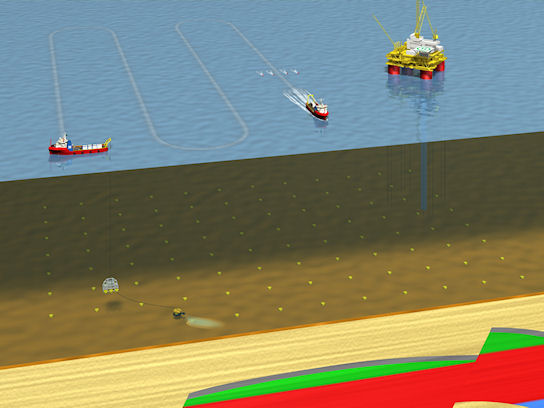
\includegraphics[height=5cm]{1_stat_models/figures/drilling}
\end{center}
\end{exampleblock}
\end{frame}

%%%%%%%%%%%%%%%%%%%%%%%%%%%%%%%%%%%%%%%%%%%%%%%%%%%%%%
\begin{frame}{}
\begin{exampleblock}{Example: Destructive tests}
\begin{center}
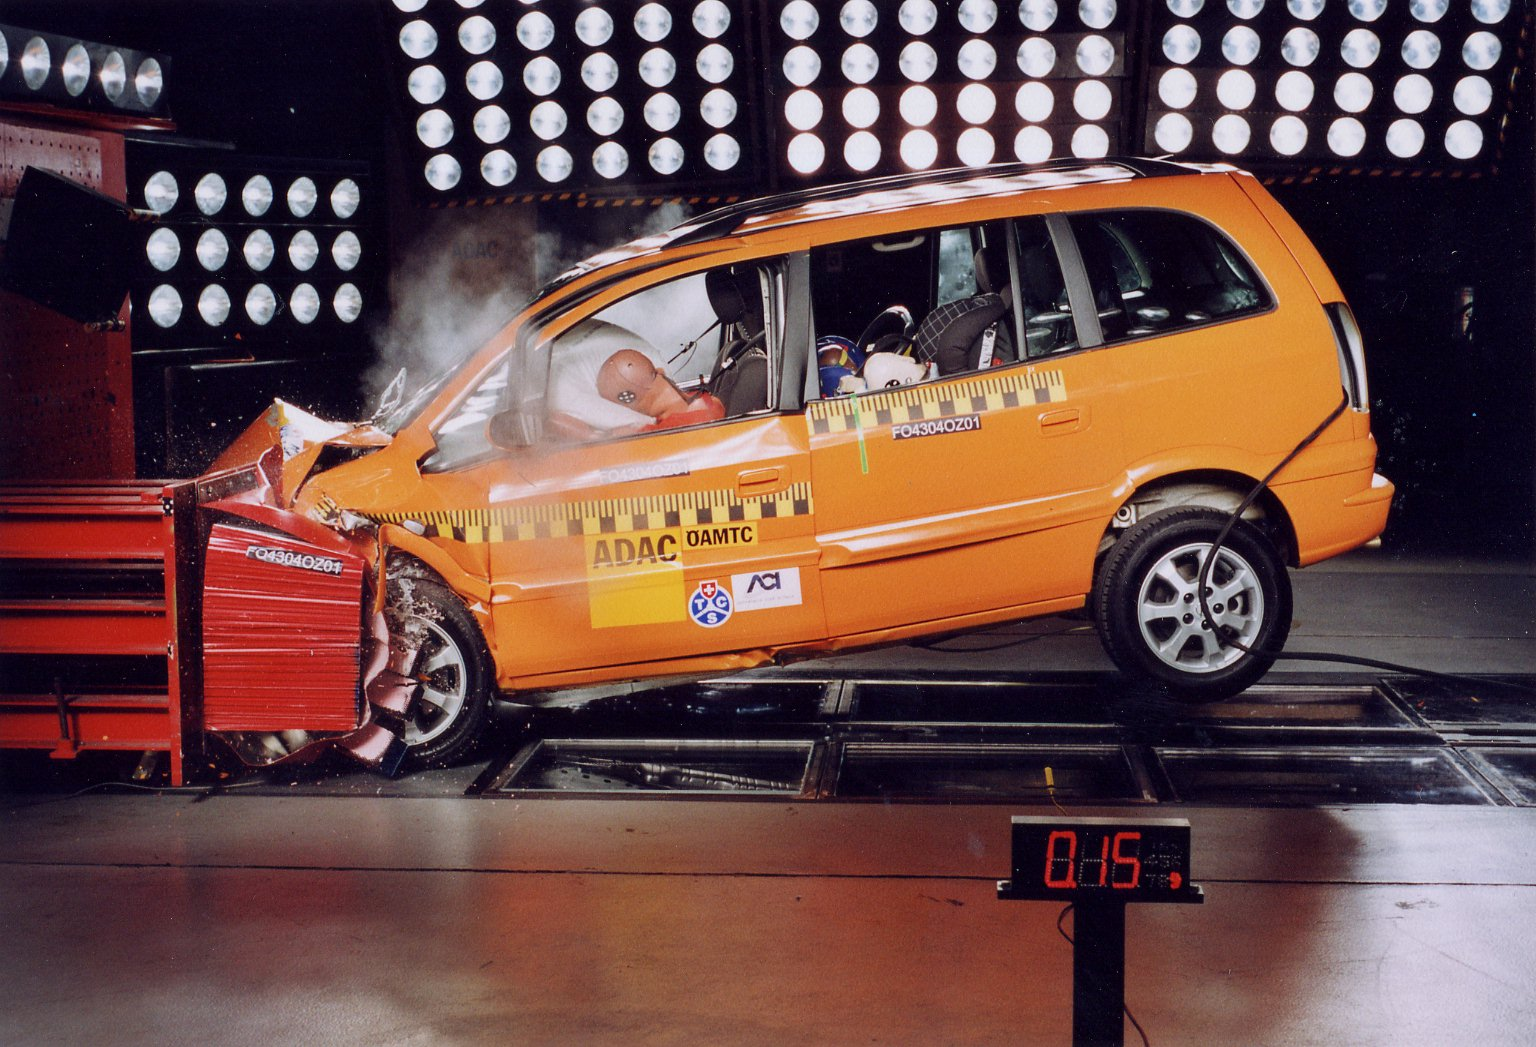
\includegraphics[height=5cm]{1_stat_models/figures/crash-test}
\end{center}
\end{exampleblock}
\end{frame}

%%%%%%%%%%%%%%%%%%%%%%%%%%%%%%%%%%%%%%%%%%%%%%%%%%%%%%
\begin{frame}{}
\begin{exampleblock}{Example: Prototyping of a boat shape}
\begin{center}
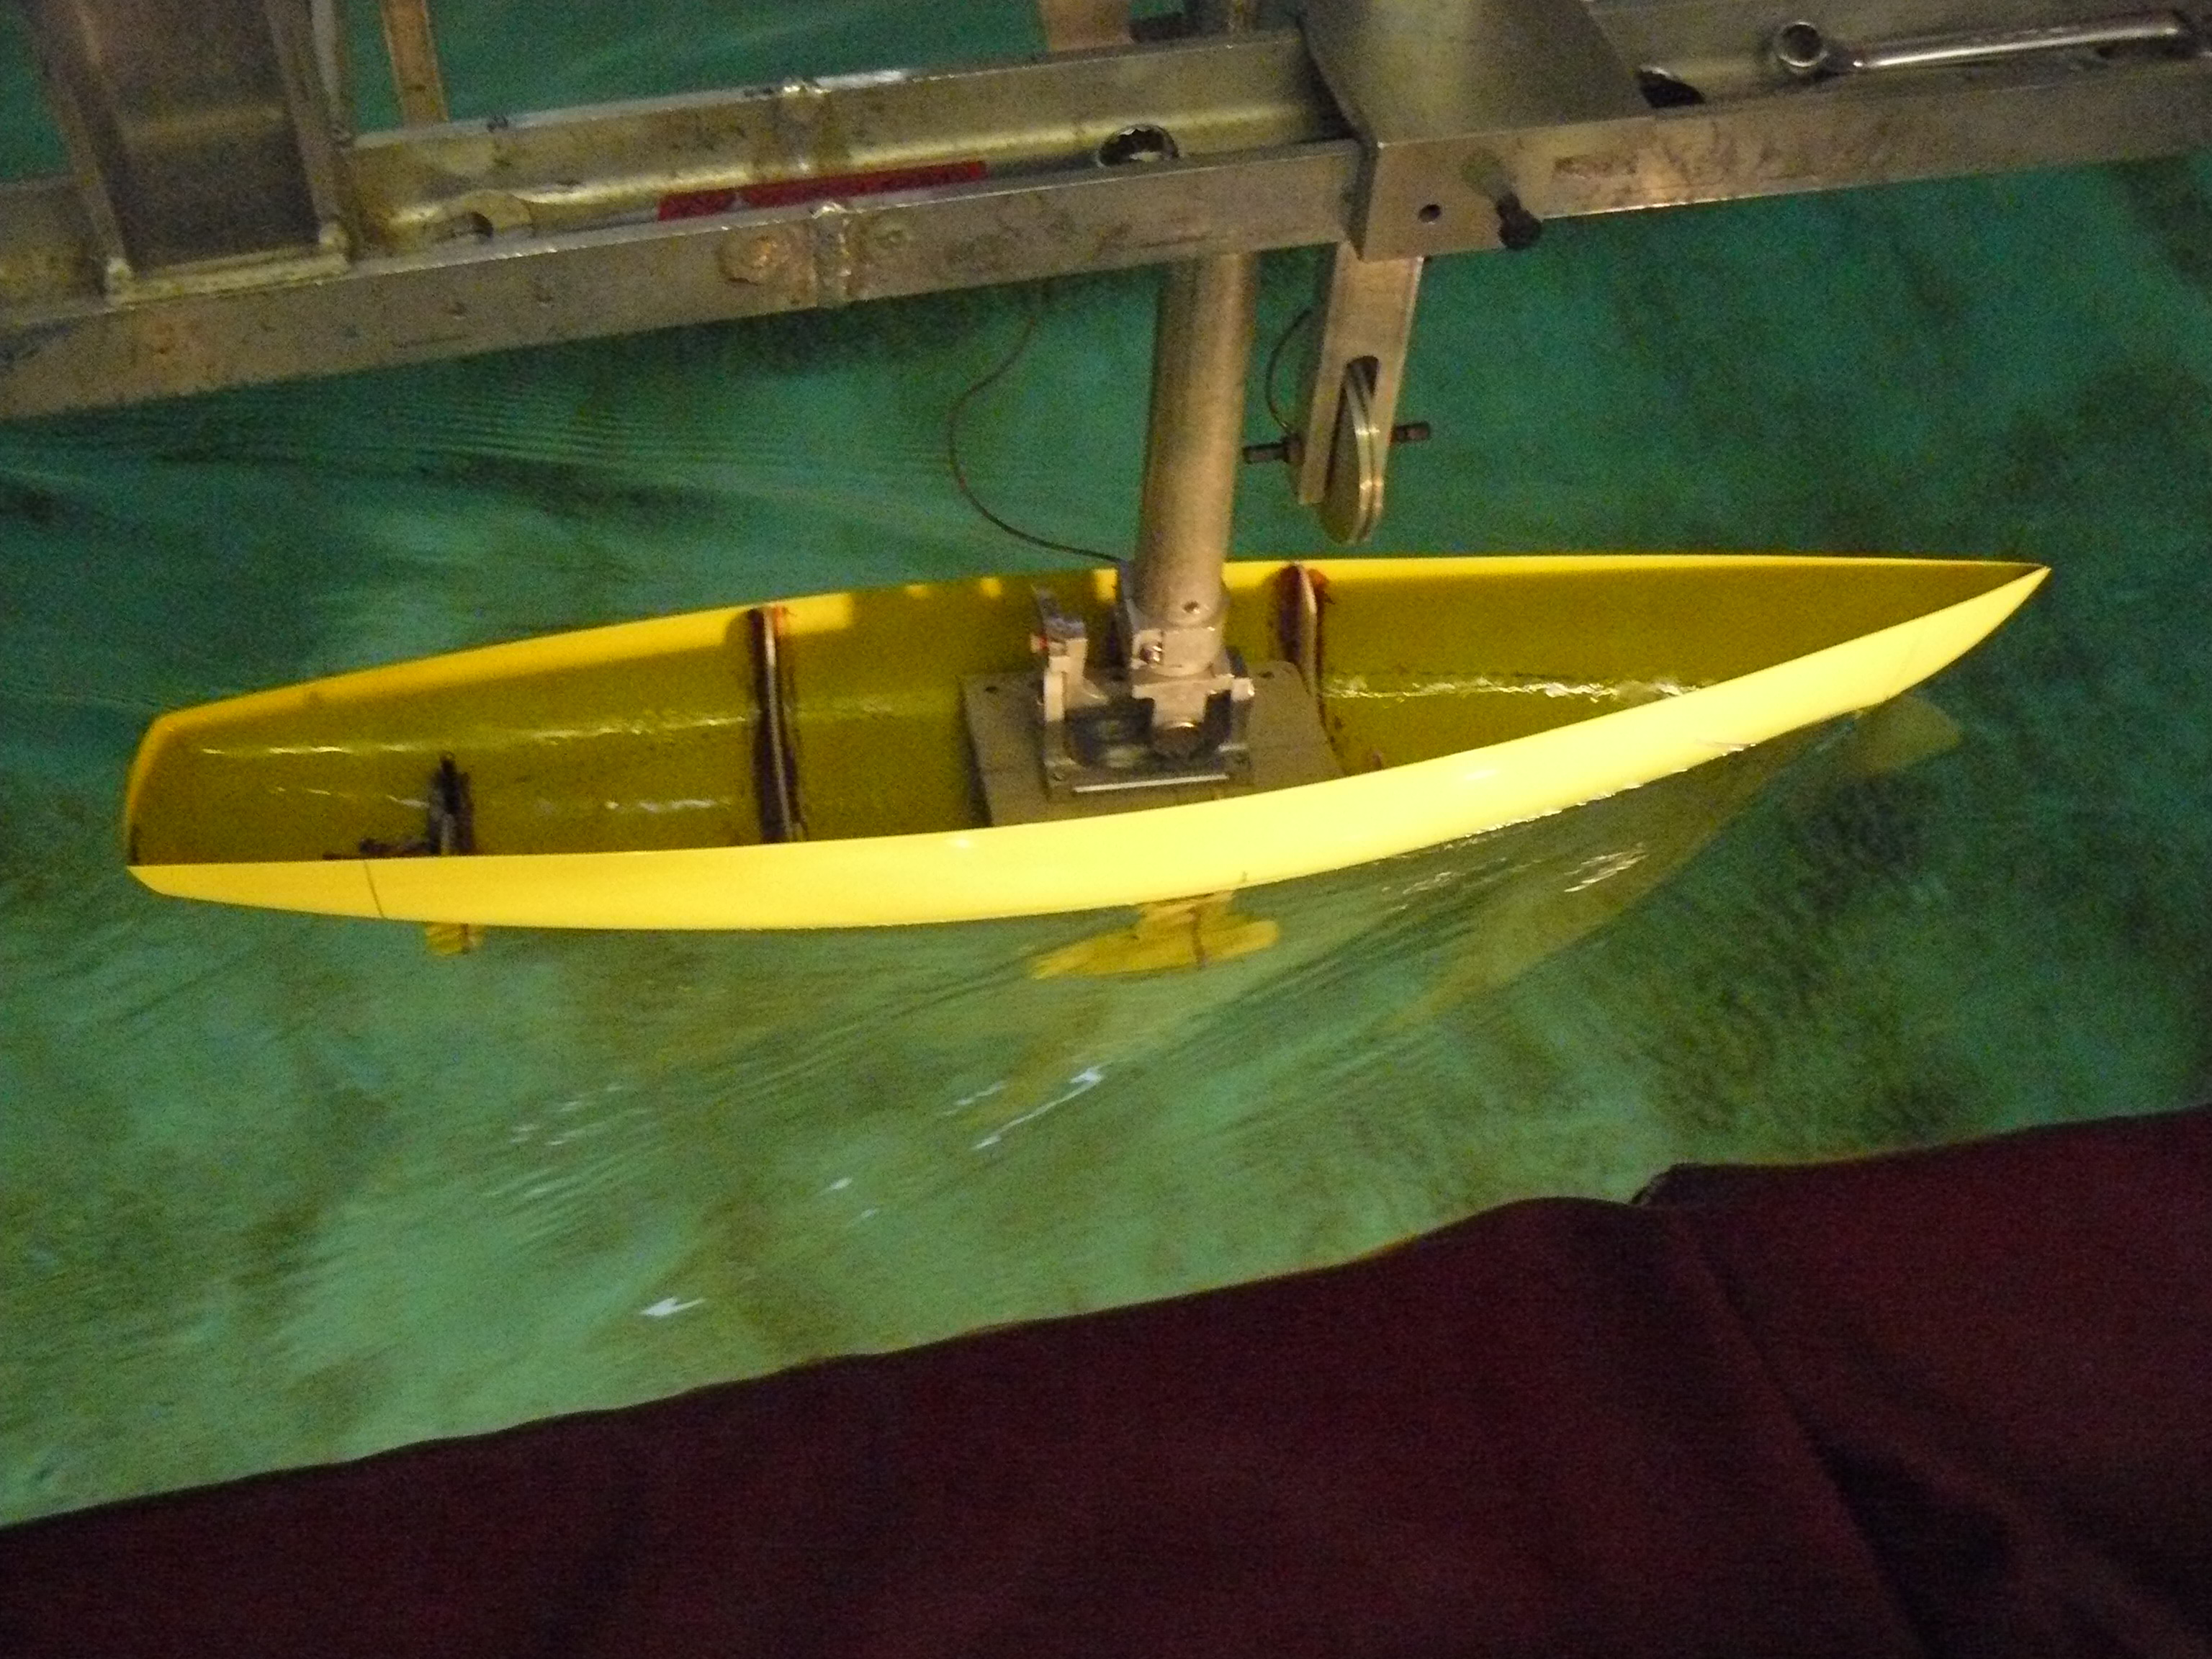
\includegraphics[height=3.5cm]{1_stat_models/figures/carene} \qquad 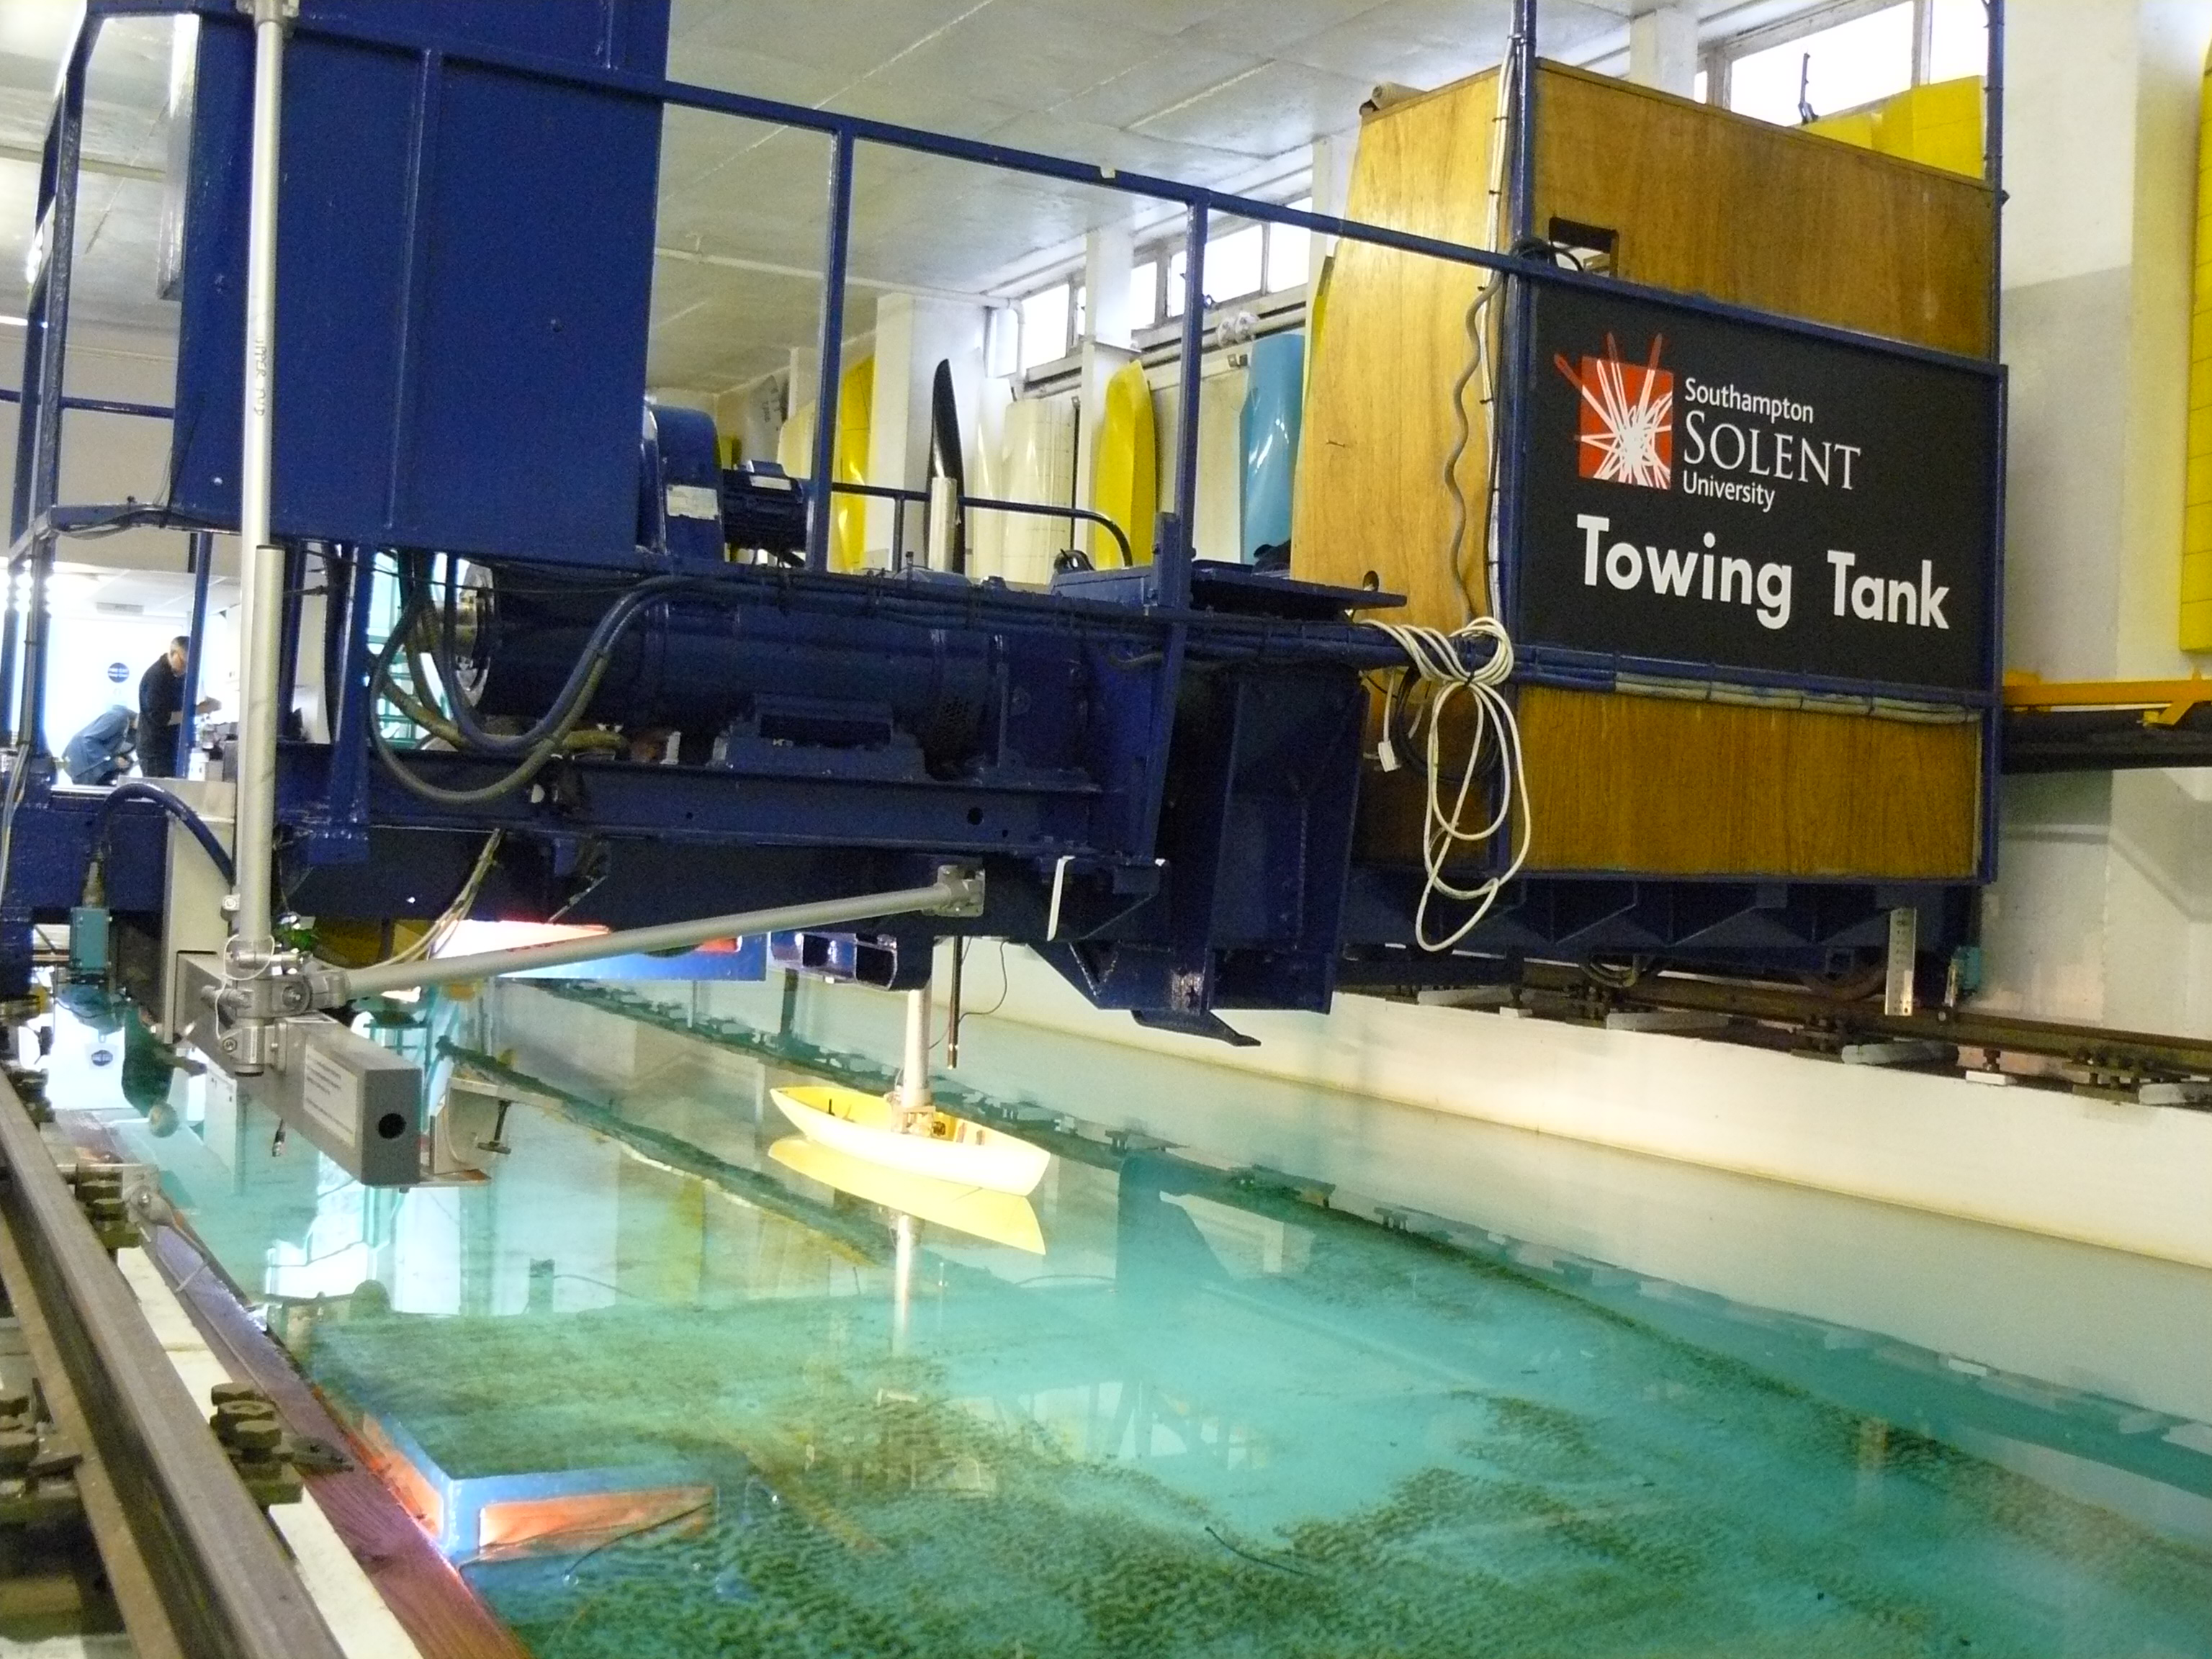
\includegraphics[height=3.5cm]{1_stat_models/figures/carene2}
\end{center}
Knowing the drag for a given design requires costly experiments
\end{exampleblock}
\end{frame}

%%%%%%%%%%%%%%%%%%%%%%%%%%%%%%%%%%%%%%%%%%%%%%%%%%%%%%
\begin{frame}{}
\begin{exampleblock}{Example: Numerical experiments}
\begin{center}
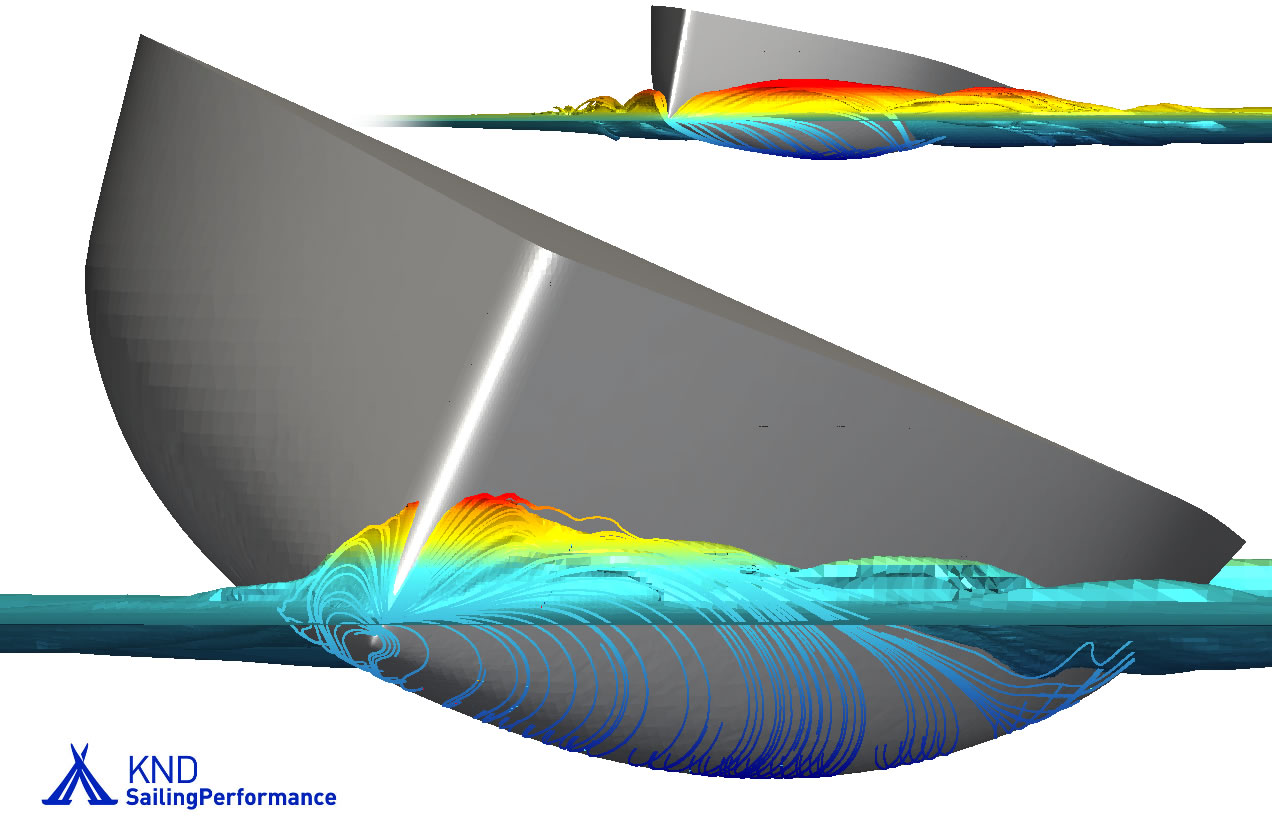
\includegraphics[height=2.8cm]{1_stat_models/figures/waterflow} \qquad 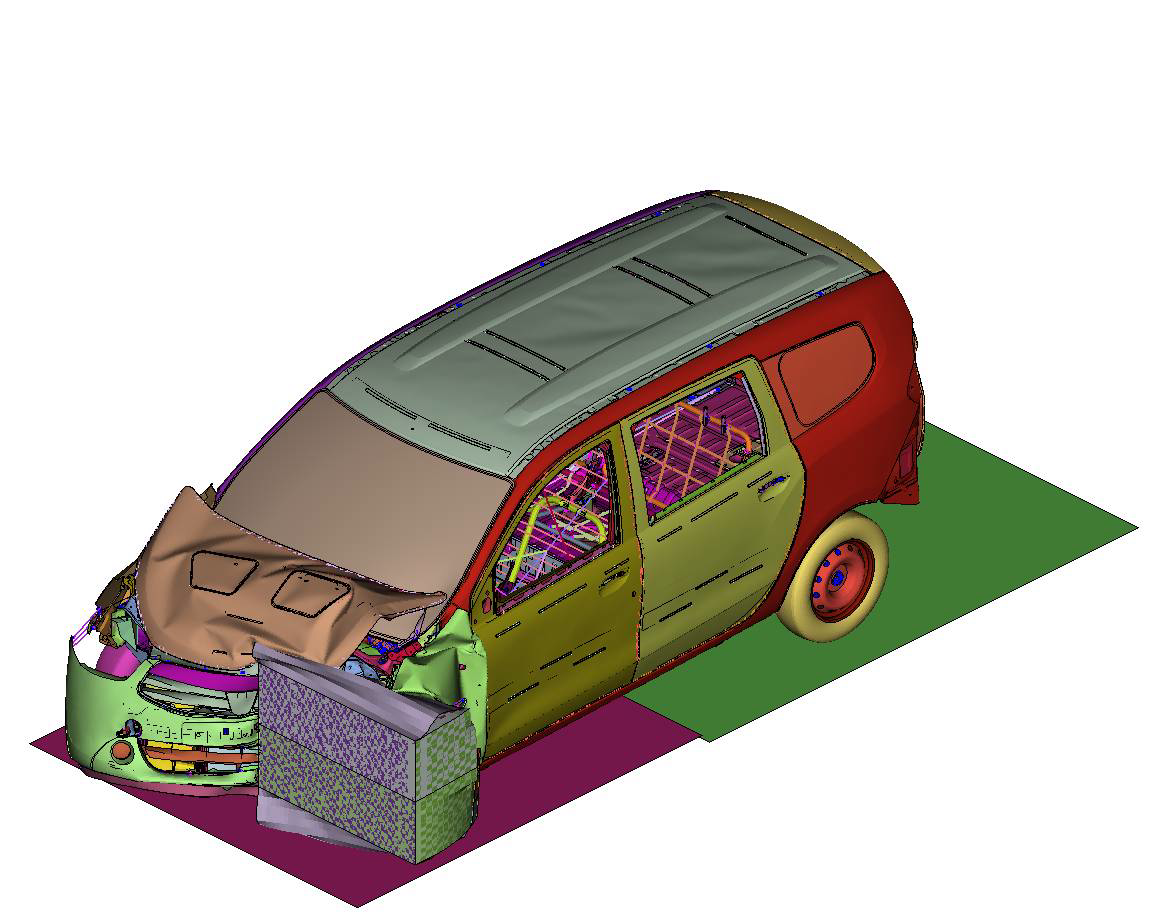
\includegraphics[height=4.2cm]{1_stat_models/figures/crash/image15}
\end{center}
Numerical experiments are less expensive but can be very time consuming!
\end{exampleblock}
\end{frame}

%%%%%%%%%%%%%%%%%%%%%%%%%%%%%%%%%%%%%%%%%%%%%%%%%%%%%%
\begin{frame}{}
In all these cases, the variable of interest can be seen as a function of the input parameters
$$ y = f(x). $$
where $f$ is a \textbf{costly to evaluate function}. \\
\vspace{5mm}
In the following, we will assume that
\begin{itemize}
	\item $x \in \mathds{R}^d$: There are many input parameters
	\item $y \in \mathds{R}$: The output is a scalar.
\end{itemize}
\end{frame}

%%%%%%%%%%%%%%%%%%%%%%%%%%%%%%%%%%%%%%%%%%%%%%%%%%%%%%
\begin{frame}{}
The fact that $f$ is \textbf{costly to evaluate} changes a lot of things...\\
\vspace{5mm}
\structure{1. Representing the function is not possible...}\\
\vspace{5mm}
\begin{center}
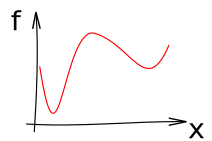
\includegraphics[height=3.2cm]{1_stat_models/figures/ink_f} 
\includegraphics[height=3.2cm]{1_stat_models/figures/Rightarrow} 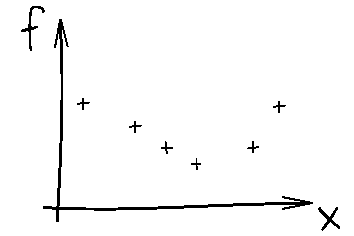
\includegraphics[height=3.2cm]{1_stat_models/figures/ink_fX}
\end{center}
\end{frame}

%%%%%%%%%%%%%%%%%%%%%%%%%%%%%%%%%%%%%%%%%%%%%%%%%%%%%%
\begin{frame}{}
The fact that $f$ is \textbf{costly to evaluate} changes a lot of things...\\
\vspace{5mm}
\structure{2. Computing integrals is not possible...}\\
\vspace{5mm}
\begin{center}
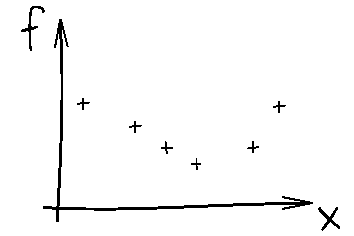
\includegraphics[height=4.5cm]{1_stat_models/figures/ink_fX}
\end{center}
What is the mean value of $f$?
\end{frame}

%%%%%%%%%%%%%%%%%%%%%%%%%%%%%%%%%%%%%%%%%%%%%%%%%%%%%%
\begin{frame}{}
The fact that $f$ is \textbf{costly to evaluate} changes a lot of things...\\
\vspace{5mm}
\structure{3. Uncertainty propagation is not possible...}\\
\vspace{5mm}
\begin{center}
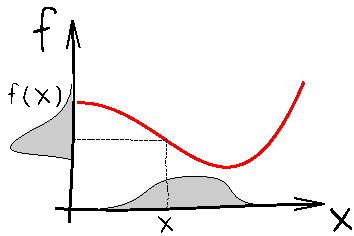
\includegraphics[height=3.2cm]{1_stat_models/figures/ink_unprogf} 
\includegraphics[height=3.2cm]{1_stat_models/figures/Rightarrow} 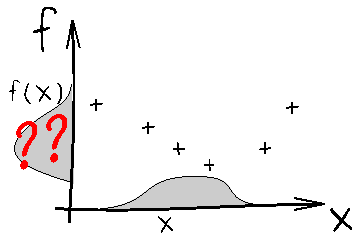
\includegraphics[height=3.2cm]{1_stat_models/figures/ink_unprogfX}
\end{center}
\end{frame}

%%%%%%%%%%%%%%%%%%%%%%%%%%%%%%%%%%%%%%%%%%%%%%%%%%%%%%
\begin{frame}{}
The fact that $f$ is \textbf{costly to evaluate} changes a lot of things...\\
\vspace{5mm}
\structure{4. Sensitivity analysis is not possible...}\\
\vspace{5mm}
\begin{center}
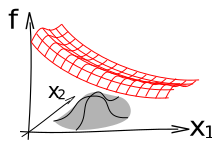
\includegraphics[height=4.5cm]{1_stat_models/figures/ink_as}
\end{center}
\end{frame}

%%%%%%%%%%%%%%%%%%%%%%%%%%%%%%%%%%%%%%%%%%%%%%%%%%%%%%
\begin{frame}{}
The fact that $f$ is \textbf{costly to evaluate} changes a lot of things...\\
\vspace{5mm}
\structure{5. Optimisation is also tricky...}\\
\vspace{5mm}
\begin{center}
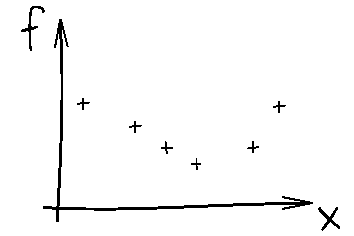
\includegraphics[height=4.5cm]{1_stat_models/figures/ink_fX}
\end{center}
\end{frame}

%%%%%%%%%%%%%%%%%%%%%%%%%%%%%%%%%%%%%%%%%%%%%%%%%%%%%%
\begin{frame}{}
The principle of statistical modelling is to use the data to build a mathematical approximation of the function.
\begin{center}
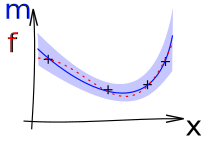
\includegraphics[height=4.5cm]{1_stat_models/figures/ink_m}
\end{center}
The model can then be used to answer all previous questions
\end{frame}

%%%%%%%%%%%%%%%%%%%%%%%%%%%%%%%%%%%%%%%%%%%%%%%%%%%%%%
\begin{frame}{}
Of course, there is a difference between $f$ and $m$...
\begin{center}
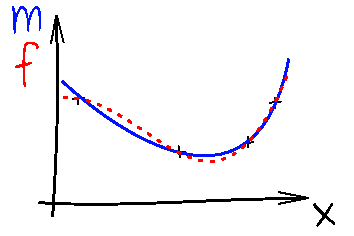
\includegraphics[height=5cm]{1_stat_models/figures/ink_mf}
\end{center}
\end{frame}

%%%%%%%%%%%%%%%%%%%%%%%%%%%%%%%%%%%%%%%%%%%%%%%%%%%%%%
\begin{frame}{}
Why \textbf{statistical models}? \\We want to be able to quantify the model error:
\begin{center}
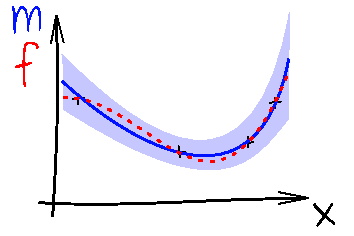
\includegraphics[height=5cm]{1_stat_models/figures/ink_mconfint}
\end{center}
The confidence intervals can be used to obtain a \textbf{measure of uncertainty on the value of interest}.
\end{frame}

%%%%%%%%%%%%%%%%%%%%%%%%%%%%%%%%%%%%%%%%%%%%%%%%%%%%%%
\begin{frame}{}
In the sequel, we will use the following notations :
\begin{itemize}
	\item The set of observation points will be represented by a $n \times d$ matrix $X=(X_1, ..., X_n)^t$
	\item The vector of observations will be denoted by $F$ : $F_i=f(X_i)$ (or $F=f(X)$).
\end{itemize}
There are many surrogate methods available on the market
\begin{itemize}
	\item Linear regression
	\item Smoothing splines
	\item Gaussian process regression
	\item Neural Networks
    \item ...
\end{itemize}
In this course we will focus on \textbf{Gaussian Process Regression}.
\end{frame}

%%%%%%%%%%%%%%%%%%%%%%%%%%%%%%%%%%%%%%%%%%%%%%%%%%%%%%
%%%%%%%%%%%%%%%%%%%%%%%%%%%%%%%%%%%%%%%%%%%%%%%%%%%%%%
\section[Gaussian Process regression]{Gaussian Process Regression}
\subsection{}
%%%%%%%%%%%%%%%%%%%%%%%%%%%%%%%%%%%%%%%%%%%%%%%%%%%%%%
\begin{frame}{}
\vspace{0.75cm}
\structure{This section is be organised in 3 subsections:}
\vspace{0.5cm}
\begin{enumerate}
    \item Univariate and multivariate normal distributions
    \item Gaussian processes
    \item Gaussian process regression
\end{enumerate}
\end{frame}

%%%%%%%%%%%%%%%%%%%%%%%%%%%%%%%%%%%%%%%%%%%%%%%%%%%%%%%%%%%%
%\subsection{Multivariate normal distribution}

%%%%%%%%%%%%%%%%%%%%%%%%%%%%%%%%%%%%%%%%%%%%%%%%%%%%%%
\begin{frame}{1D normal distribution}
We say that $X \sim \mathcal{N}(\mu,\sigma^2)$ if it has the following pdf:
\begin{columns}
  \begin{column}{0.6\textwidth}
  \begin{equation*}
  f(x) = \frac{1}{\sigma \sqrt{2 \pi}} \exp \left(-\frac{(x-\mu)^2}{2 \sigma^2} \right)
  \vspace{3mm}
  \end{equation*}
  The distribution is characterised by\\
      \qquad mean: $\mu = \E [X]$\\
      \qquad variance: $\sigma^2 = \E [X^2] - \E[X]^2$
  \end{column}
  \begin{column}{0.5\textwidth}
  \begin{center}
   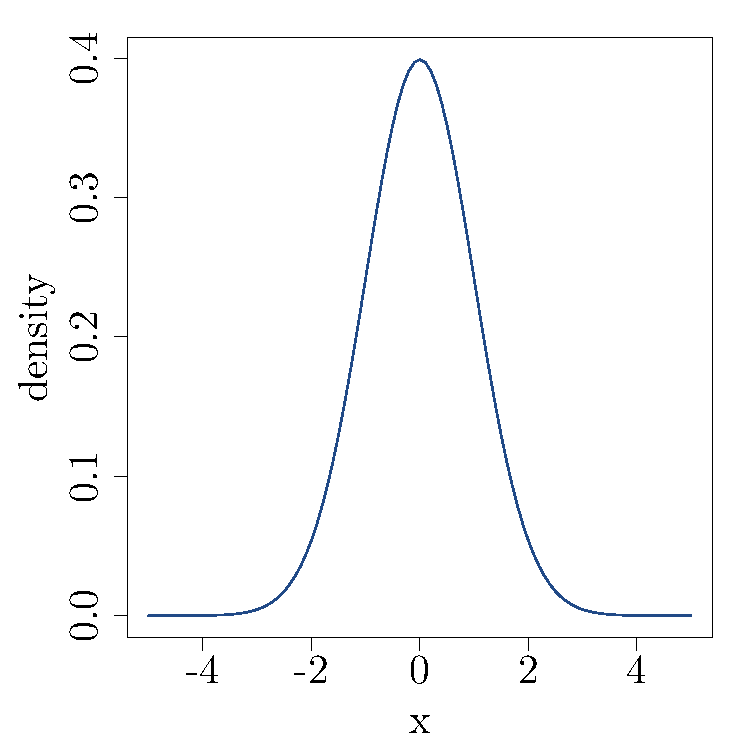
\includegraphics[height=4.7cm]{1_stat_models/figures/R/MVN_dens1} 
  \end{center}
  \end{column}
\end{columns}
\vspace{2mm}
\structure{One fundamental property:} a linear combination of independant normal distributed random variables is still normal distributed.
\end{frame}

%%%%%%%%%%%%%%%%%%%%%%%%%%%%%%%%%%%%%%%%%%%%%%%%%%%%%%
\begin{frame}{Multivariate normal distribution}
\begin{definition}
	We say that a vector $Y=(Y_1, \dots, Y_d)^t$ follows a multivariate normal distribution if any linear combination of $Y$ follows a normal distribution:
	\begin{equation*}
		\forall \alpha \in \mathds{R}^d,\ \alpha^t Y \sim \mathcal{N}
	\end{equation*}
\end{definition}
The distribution of a Gaussian vector is characterised by
\begin{itemize}
 	\item a \textbf{mean vector} $\mu = \E [Y]$
 	\item a \textbf{covariance matrix} $\Sigma = \E[YY^t] - \E[Y] \E[Y]^t$ % \hfill (i.e. $\Sigma_{i,j}=\Cov(Y_i, Y_j)$)
\end{itemize}
\vspace{3mm}
\structure{Property:}\\
A covariance matrix is
\begin{itemize}
	\item symmetric $K_{i,j}=K_{j,i}$
	\item positive semi-definite $\forall \alpha \in \mathds{R}^d, \alpha^t K \alpha \geq 0$.
\end{itemize}
\end{frame}

%%%%%%%%%%%%%%%%%%%%%%%%%%%%%%%%%%%%%%%%%%%%%%%%%%%%%%
\begin{frame}{}
The density of a multivariate Gaussian is:
\begin{equation*}
f_Y(x) = \frac{1}{\displaystyle (2 \pi)^{d/2} |\Sigma|^{1/2}} \exp \left(-\frac12 (x-\mu)^t \Sigma^{-1} (x-\mu)  \right).
\end{equation*}
\begin{center}
 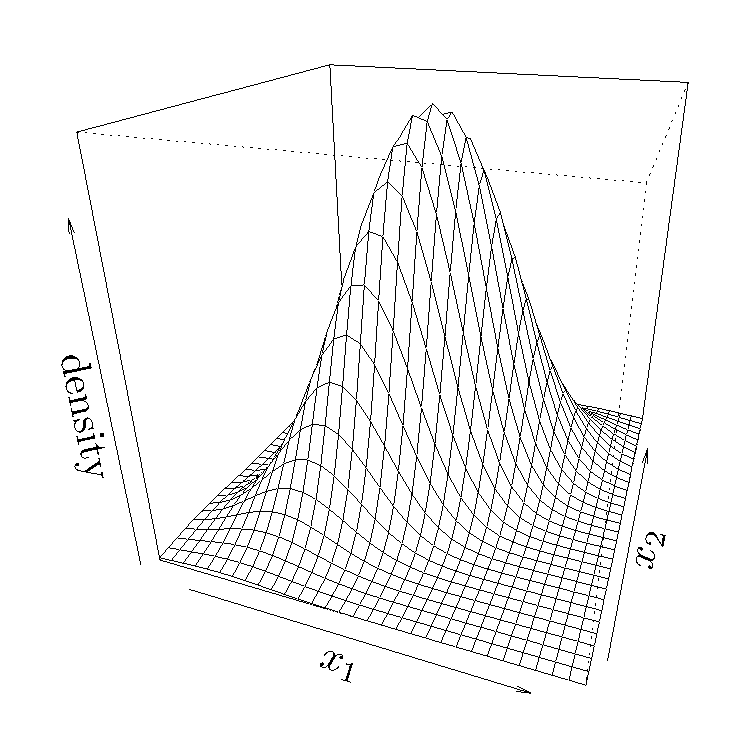
\includegraphics[height=5cm]{1_stat_models/figures/R/MVN_dens2}
\end{center}
\end{frame}


%%%%%%%%%%%%%%%%%%%%%%%%%%%%%%%%%%%%%%%%%%%%%%%%%%%%%%
\begin{frame}{}
\begin{exampleblock}{Samples from a multivariate normal}
 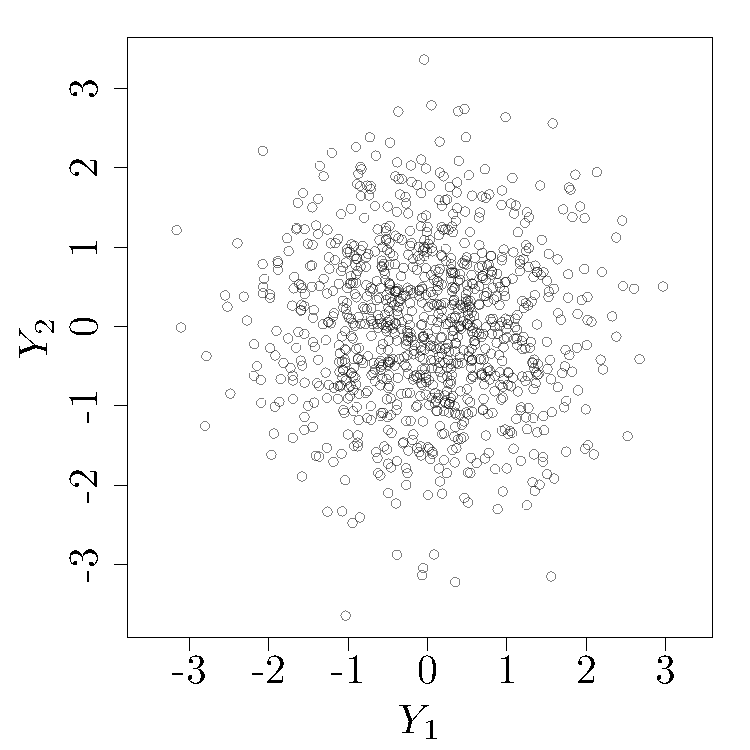
\includegraphics[height=5cm]{1_stat_models/figures/R/MVN_gaussvec2} \quad 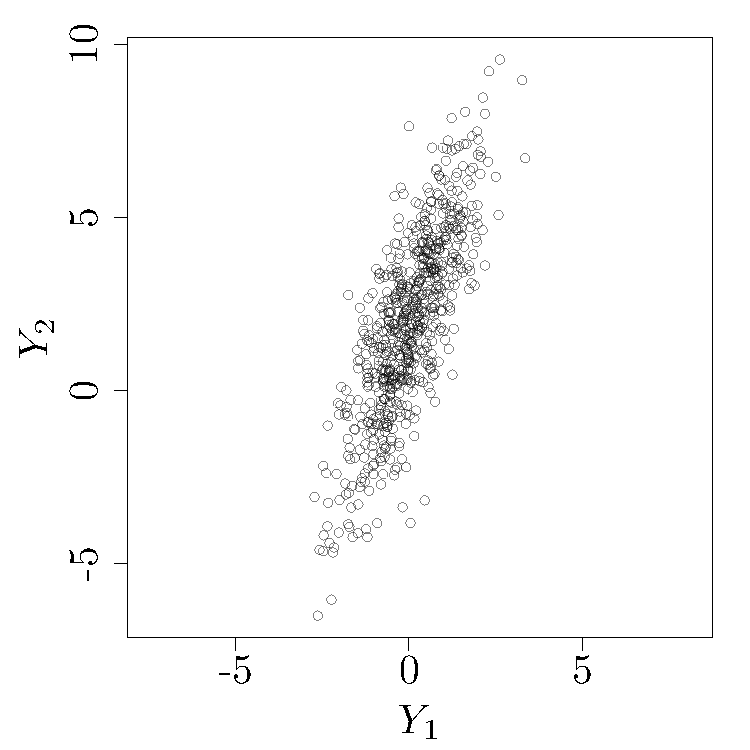
\includegraphics[height=5cm]{1_stat_models/figures/R/MVN_gaussvec1}
\end{exampleblock}
\vspace{-5mm}
\begin{exampleblock}{Exercise}
\begin{itemize}
  \item For $X=(X_1,\dots,X_d)$ with $X_i$ independant and $\mathcal{N}(0,1)$, and a $d \times d$ matrix $A$, what is the distribution of $AX$?
  \item For a given covariance matrix $K$ and independant $\mathcal{N}(0,1)$ samples, how can we generate $\mathcal{N}(\mu,K)$ random samples?
\end{itemize}
\end{exampleblock}
\end{frame}

%%%%%%%%%%%%%%%%%%%%%%%%%%%%%%%%%%%%%%%%%%%%%%%%%%%%%%
\begin{frame}{}
\begin{exampleblock}{Counter example}
\begin{center}
 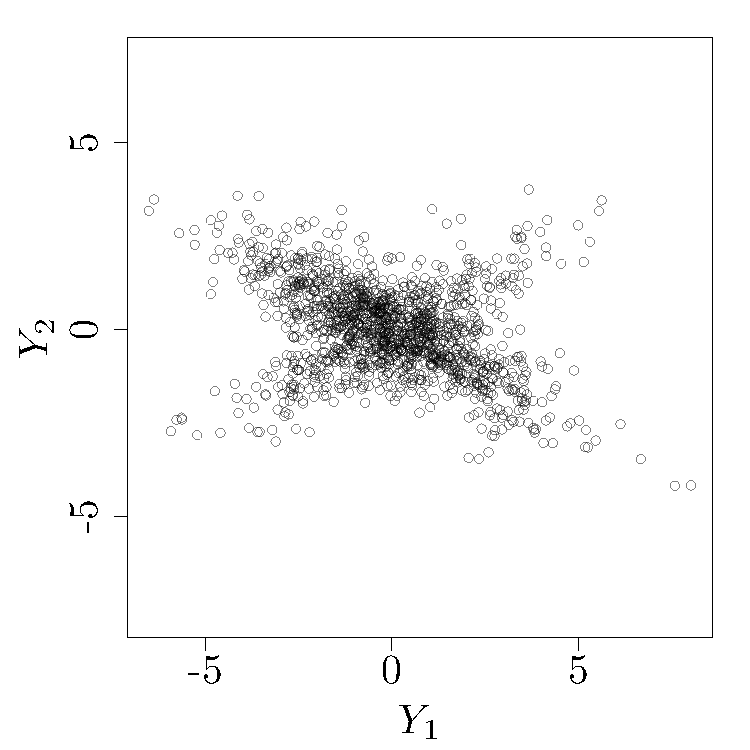
\includegraphics[height=5cm]{1_stat_models/figures/R/MVN_gaussvec3}
\end{center}
$Y_1$ and $Y_2$ are normally distributed but \textbf{the couple $(Y_1,Y_2)$ is not}.
\end{exampleblock}
\end{frame}


%%%%%%%%%%%%%%%%%%%%%%%%%%%%%%%%%%%%%%%%%%%%%%%%%%%%%%
\begin{frame}{}
\begin{block}{Conditional distribution}
Let $(Y,Z)$ be a Gaussian vector ($Y$ and $Z$ may both be vectors) with mean $(\mu_Y,\mu_Z)^t$ and covariance matrix
\begin{equation*}
\begin{pmatrix}
	\Cov(Y,Y) & \Cov(Y,Z)\\
	\Cov(Z,Y) & \Cov(Z,Z)\\
\end{pmatrix}.
\end{equation*}
The conditional distribution of $Y$ knowing $Z$ is still multivariate normal $Y|Z \sim \mathcal{N}(\mu_{cond},\Sigma_{cond})$ with
\begin{equation*}
\begin{split}
	\mu_{cond} &= \E [Y|Z] = \mu_Y + \Cov(Y,Z) \Cov(Z,Z)^{-1} (Z-\mu_Z)\\
	\Sigma_{cond} &= \Cov [Y,Y|Z] = \Cov(Y,Y) - \Cov(Y,Z) \Cov(Z,Z)^{-1} \Cov(Z,Y)
\end{split}
\end{equation*}
\end{block}
\end{frame}

%%%%%%%%%%%%%%%%%%%%%%%%%%%%%%%%%%%%%%%%%%%%%%%%%%%%%%
\begin{frame}{}
\begin{exampleblock}{Example 1}
2D multivariate Gaussian conditional distribution:\\
\begin{center}
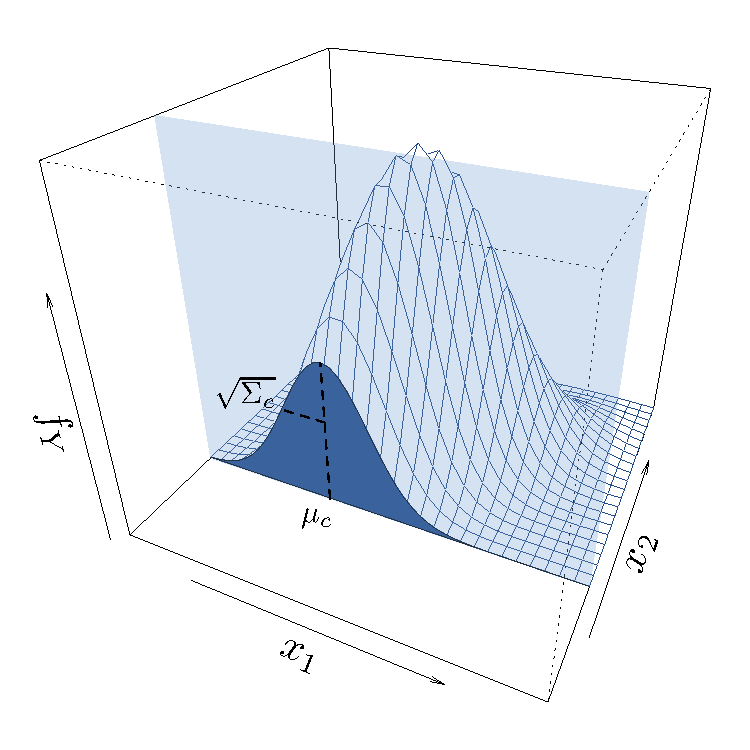
\includegraphics[height=6cm]{1_stat_models/figures/ch1_condpdf1}
\end{center}
\end{exampleblock}
\end{frame}

%%%%%%%%%%%%%%%%%%%%%%%%%%%%%%%%%%%%%%%%%%%%%%%%%%%%%%
\begin{frame}{}
\begin{exampleblock}{Example 2}
3D multivariate Gaussian conditional distribution:\\
\begin{center}
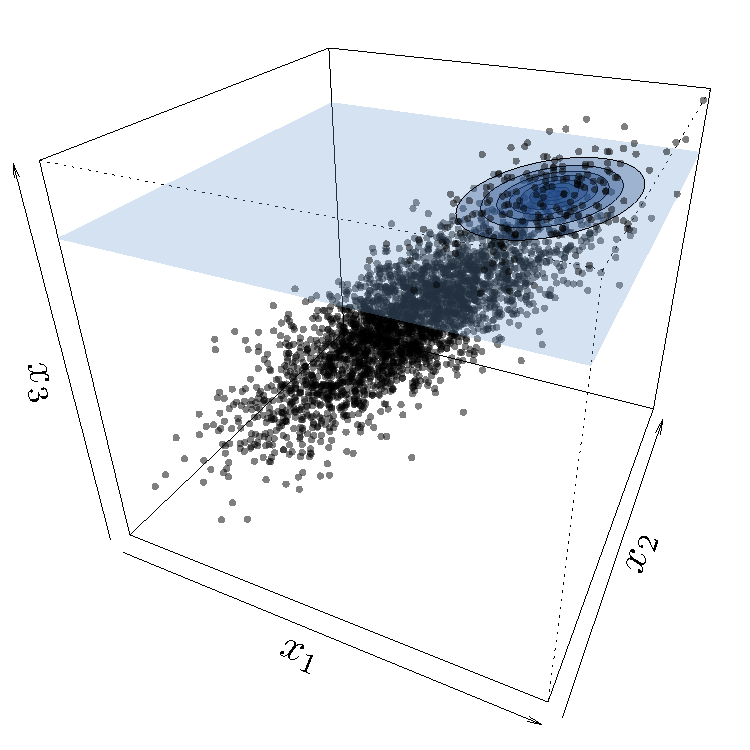
\includegraphics[height=6cm]{1_stat_models/figures/ch1_condpdf2}
\end{center}
\end{exampleblock}
\end{frame}



%%%%%%%%%%%%%%%%%%%%%%%%%%%%%%%%%%%%%%%%%%%%%%%%%%%%%%
\begin{frame}{2. Gaussian processes}
The multivariate Gaussian distribution can be generalised to random processes:
\begin{definition}
A random process $Z$ over $D \subset \mathds{R}^d$ is said to be Gaussian if
\begin{equation*}
\forall n \in \mathds{N}, \forall x_i \in D, (Z(x_1),\dots,Z(x_n)) \text{  is a Gaussian vector}.
\end{equation*}
\end{definition}
The distribution of a GP is fully characterised by:
\begin{itemize}
	\item its mean function $m$ defined over $D$
	\item its covariance function (or kernel) $k$ defined over $D \times D$: $k(x,y) = \Cov(Z(x),Z(y))$
\end{itemize}
We will use the notation $Z \sim \mathcal{N}(m(.),k(.,.))$.
\end{frame}

%%%%%%%%%%%%%%%%%%%%%%%%%%%%%%%%%%%%%%%%%%%%%%%%%%%%%%
\begin{frame}{}
A kernel satisfies the following properties:
\begin{itemize}
	\item It is symmetric: $k(x,y) = k(y,x)$
	\item It is positive semi-definite (psd):
\end{itemize}
\begin{equation*}
	\forall n \in \mathds{N}, \forall x_i \in D, \forall \alpha \in \mathds{R}^n,\  \sum_{i=1}^n \sum_{j=1}^n \alpha_i \alpha_j k(x_i,x_j) \geq 0
\end{equation*}
\vspace{5mm} \\
Furthermore any symmetric psd function can be seen as the covariance of a Gaussian process. This equivalence is known as the Loeve theorem.
\end{frame}

%%%%%%%%%%%%%%%%%%%%%%%%%%%%%%%%%%%%%%%%%%%%%%%%%%%%%%
\begin{frame}{}
There are a lot of functions that have already been proven psd:\\
\vspace{2mm}
\footnotesize
\begin{tabular}{rlN}
		constant & $ \displaystyle k(x,y) = \sigma^2 $ &\\[4mm]
		white noise & $ \displaystyle k(x,y) = \sigma^2 \delta_{x,y} $ &\\[4mm]
		Brownian & $ \displaystyle k(x,y) =  \sigma^2  \min (x,y) $ &\\[4mm]
		exponential & $\displaystyle k(x,y) =  \sigma^2 \exp \left(- |x-y|/\theta \right)$ &\\[4mm]
		Matern 3/2 & $\displaystyle k(x,y) =  \sigma^2 \left(1 + |x-y| \right) \exp \left(- |x-y| /\theta\right)$ &\\[4mm]
		Matern 5/2 & $\displaystyle k(x,y) =  \sigma^2 \left(1 + |x-y| /\theta+ 1/3|x-y|^2 /\theta^2 \right) \exp \left(- |x-y| /\theta\right)$ &\\[4mm]
		\hspace{-5mm}squared exponential & $\displaystyle k(x,y) =  \sigma^2 \exp \left(- (x-y)^2 /\theta^2 \right)$ &\\[4mm]
		$\vdots$ &
		% linear & $ \displaystyle k(x,y) = \sigma^2 xy $ &\\[4mm]
		% cosine & $ \displaystyle k(x,y) = \sigma^2 \cos \left (\frac{x-y}{\theta} \right) $ &\\[4mm]
		% sinc & $ \displaystyle k(x,y) = \sigma^2 \frac{\theta}{x-y} \sin \left( \frac{x-y}{\theta} \right) $ &\\[4mm] \hline
\end{tabular}\\
%%\begin{tabular}{rlN}
%%		constant & $ \displaystyle k(x,y) = 1 $ &\\[4mm]
%%		white noise & $ \displaystyle k(x,y) = \delta_{x,y} $ &\\[4mm]
%%		Brownian & $ \displaystyle k(x,y) =  \min (x,y) $ &\\[4mm]
%%		exponential & $\displaystyle k(x,y) = \exp \left(- |x-y| \right)$ &\\[4mm]
%%		Matern 3/2 & $\displaystyle k(x,y) = \left(1 + |x-y| \right) \exp \left(- |x-y| \right)$ &\\[4mm]
%%		Matern 5/2 & $\displaystyle k(x,y) = \left(1 + |x-y| + 1/3|x-y|^2 \right) \exp \left(- |x-y| \right)$ &\\[4mm]
%%		squared exponential & $\displaystyle k(x,y) = \exp \left(- (x-y)^2 \right)$ &\\[4mm]
%%		$\vdots$ &
%%		% linear & $ \displaystyle k(x,y) = \sigma^2 xy $ &\\[4mm]
%%		% cosine & $ \displaystyle k(x,y) = \sigma^2 \cos \left (\frac{x-y}{\theta} \right) $ &\\[4mm]
%%		% sinc & $ \displaystyle k(x,y) = \sigma^2 \frac{\theta}{x-y} \sin \left( \frac{x-y}{\theta} \right) $ &\\[4mm] \hline
%%\end{tabular}\\
\vspace{2mm}
\normalsize
When $k$ is a function of $x-y$, the kernel is called \textbf{stationary}. \\
The parameter $\sigma^2$ is called the \textbf{variance} and $\theta$ the \textbf{length-scale}.
\end{frame}

%%%%%%%%%%%%%%%%%%%%%%%%%%%%%%%%%%%%%%%%%%%%%%%%%%%%%%
\begin{frame}{}
Can we look at the sample paths associated to these kernels?\\
\vspace{5mm}
In order to simulate sample paths from a GP $Z \sim \mathcal{N}(m(.),k(.,.))$, we will consider samples of the GP discretised on a fine grid.
\vspace{5mm}
\begin{exampleblock}{Exercise: Simulating sample paths}
Let X be a set 100 regularly spaced points over the input space of $Z$.
\begin{itemize}
	\item What is the distribution of $Z(X)$ ?
	\item How to simulate samples from $Z(X)$ ?
\end{itemize}
\end{exampleblock}
\vspace{5mm}
$\Rightarrow$ Shiny App: \url{https://github.com/NicolasDurrande/shinyApps}
\end{frame}

%%%%%%%%%%%%%%%%%%%%%%%%%%%%%%%%%%%%%%%%%%%%%%%%%%%%%%
\begin{frame}{}
In higher dimension one can introduce one length-scale parameter per dimension. The usual Euclidean distance between two points $|| x-y || = ( \sum (x_i-y_i)^2)^{1/2}$ is thus replaced by
\begin{equation*}
	\Ni{x-y}{\theta} = \left( \sum_{i=1}^d \frac{(x_i-y_i)^2}{\theta_i^2} \right)^{1/2}.
\end{equation*}
If the parameters $\theta_i$ are equal for all the dimensions, the covariance (or the process) is called \textbf{isotropic}.
\end{frame}

%%%%%%%%%%%%%%%%%%%%%%%%%%%%%%%%%%%%%%%%%%%%%%%%%%%%%%
\begin{frame}{}
Here is a list of the most common kernels:\\
\vspace{2mm}
\footnotesize
\centering
\begin{tabular}{rlN}
		constant & $ \displaystyle k(x,y) = \sigma^2 $ &\\[4mm]
		white noise & $ \displaystyle k(x,y) = \sigma^2 \delta_{x,y} $ &\\[4mm]
		exponential & $\displaystyle k(x,y) = \sigma^2 \exp \left(- \Ni{x-y}{\theta} \right)$ &\\[4mm]
		Matern 3/2 & $\displaystyle k(x,y) = \sigma^2 \left(1 + \sqrt{3}\Ni{x-y}{\theta} \right) \exp \left(- \sqrt{3}\Ni{x-y}{\theta}  \right)$ &\\[4mm]
		Matern 5/2 & $\displaystyle k(x,y) = \sigma^2 \left(1 + \sqrt{5}\Ni{x-y}{\theta} + \frac{5}{3}\Ni{x-y}{\theta}^2 \right) \exp \left(- \sqrt{5}\Ni{x-y}{\theta} \right)$ &\\[4mm]
		Gaussian & $\displaystyle k(x,y) = \sigma^2 \exp \left(- \frac12 \Ni{x-y}{\theta}^2 \right)$ &\\[4mm]
\end{tabular}
\end{frame}

%%%%%%%%%%%%%%%%%%%%%%%%%%%%%%%%%%%%%%%%%%%%%%%%%%%%%%%%%%%%
%\subsection{Gaussian process regression}

%%%%%%%%%%%%%%%%%%%%%%%%%%%%%%%%%%%%%%%%%%%%%%%%%%%%%%
\begin{frame}{3. Gaussian process regression}
We assume we have observed a function $f$ for a set of points $X = (X_1,\dots,X_n)$:
\begin{center}
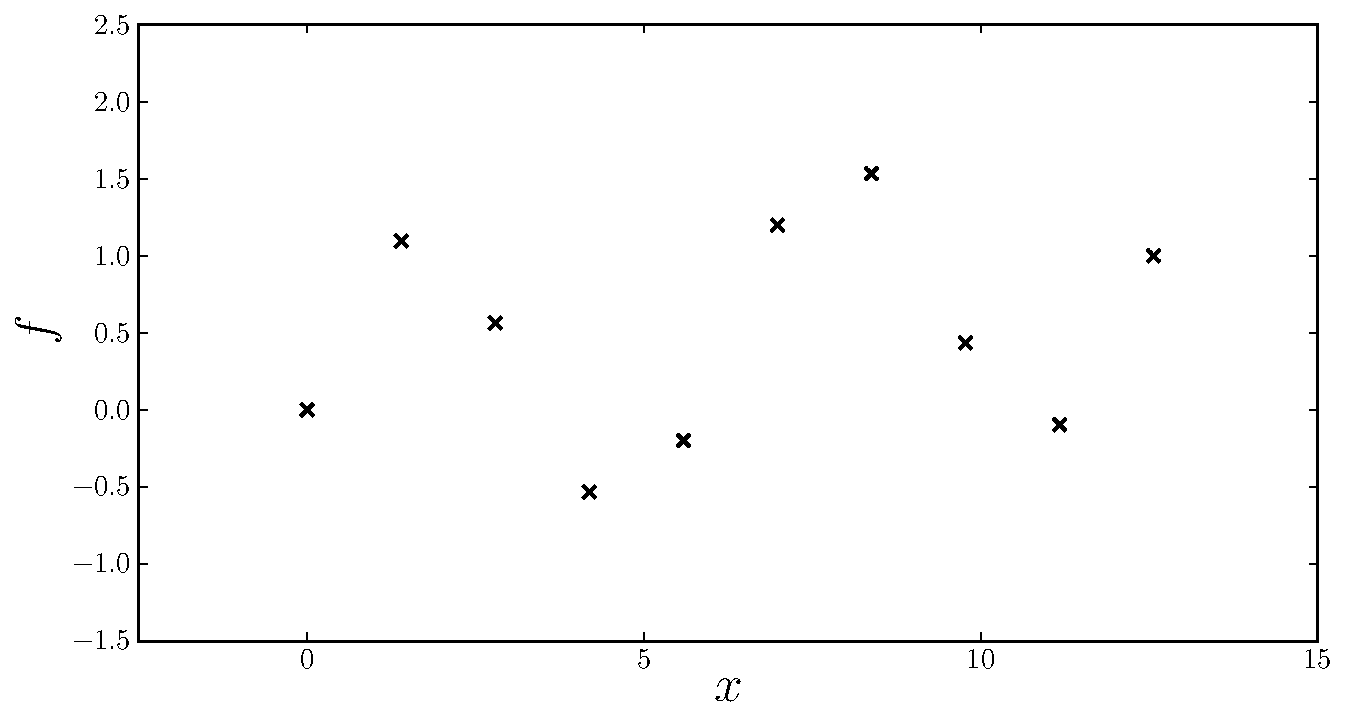
\includegraphics[height=5cm]{1_stat_models/figures/R/Fig1-data}
\end{center}
The vector of observations is $F=f(X)$ (ie $F_i = f(X_i)$ ).
\end{frame}

%%%%%%%%%%%%%%%%%%%%%%%%%%%%%%%%%%%%%%%%%%%%%%%%%%%%%%
\begin{frame}{}
Since $f$ in unknown, we make the general assumption that
it is the sample path of a Gaussian process $Z \sim \mathcal{N}(0,k)$:
\begin{center}
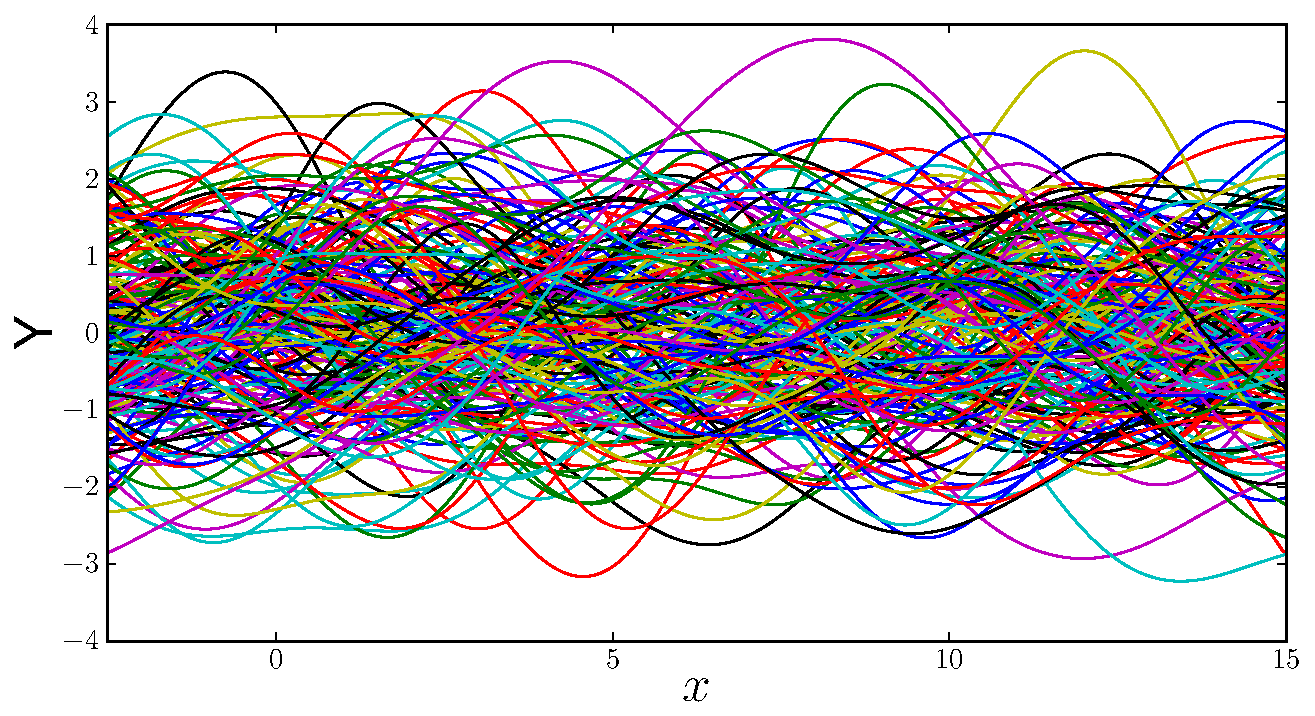
\includegraphics[height=5cm]{1_stat_models/figures/R/Fig1b-sim}
\end{center}
What would be the next step?
\end{frame}

%%%%%%%%%%%%%%%%%%%%%%%%%%%%%%%%%%%%%%%%%%%%%%%%%%%%%%
\begin{frame}{}
We can look at the conditional distribution of $Z$ knowing that it interpolates the data points:
\begin{exampleblock}{Exercise}
\begin{itemize}
	\item[1.] What is the conditional distribution of $Z(x)|Z(X)=F$?
	\item[2.] Compute the conditional mean $m$ and covariance $c(.,.)$.
	\item[3.] Compute $m(X_1)$ and $c(X_1,X_1)$.
\end{itemize}
\end{exampleblock}
\end{frame}

%%%%%%%%%%%%%%%%%%%%%%%%%%%%%%%%%%%%%%%%%%%%%%%%%%%%%%
\begin{frame}{}
\begin{exampleblock}{Solution}
	\begin{itemize}
		\item[1.] The conditional distribution is Gaussian.
		\item[2.] It has mean and variance
			\begin{equation*}
			\begin{split}
				m(x) &= \E[Z(x)|Z(X) \shorteq F] \\
				&= k(x,X) k(X,X)^{-1} F \\ \vspace{3mm}
				c(x,y) &= \Cov[Z(x),Z(y)|Z(X) \shorteq F] \\
				&= k(x,y) - k(x,X) k(X,X)^{-1} k(X,y)
			\end{split}
			\end{equation*}
		\item[3.] We have $m(X_1)=F_1$ and $c(X_1,X_1)=0$
		\end{itemize}
\end{exampleblock}
\end{frame}


%%%%%%%%%%%%%%%%%%%%%%%%%%%%%%%%%%%%%%%%%%%%%%%%%%%%%%
\begin{frame}{}
We can look at sample paths from the conditional distribution
\begin{center}
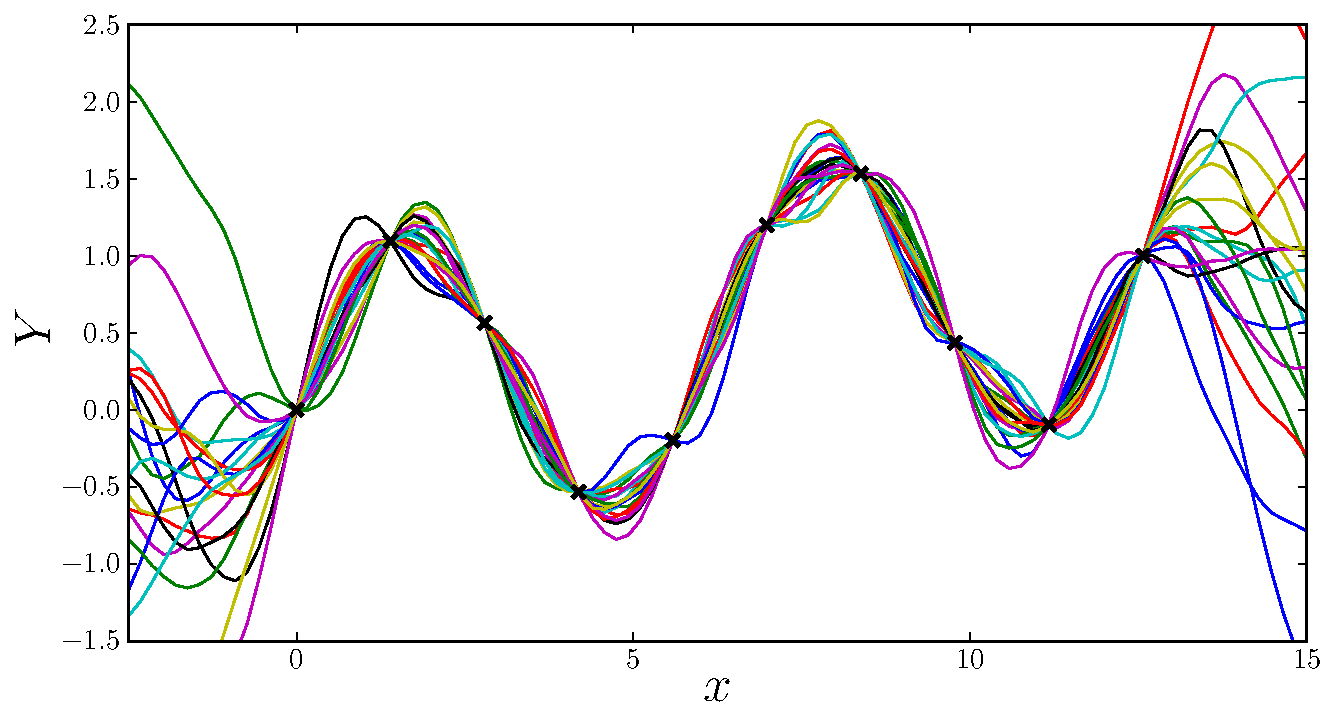
\includegraphics[height=6cm]{1_stat_models/figures/R/Fig1-sim-cond}
\end{center}
\end{frame}

%%%%%%%%%%%%%%%%%%%%%%%%%%%%%%%%%%%%%%%%%%%%%%%%%%%%%%
\begin{frame}{}
It can summarized by a mean function and 95\% confidence intervals.
\begin{center}
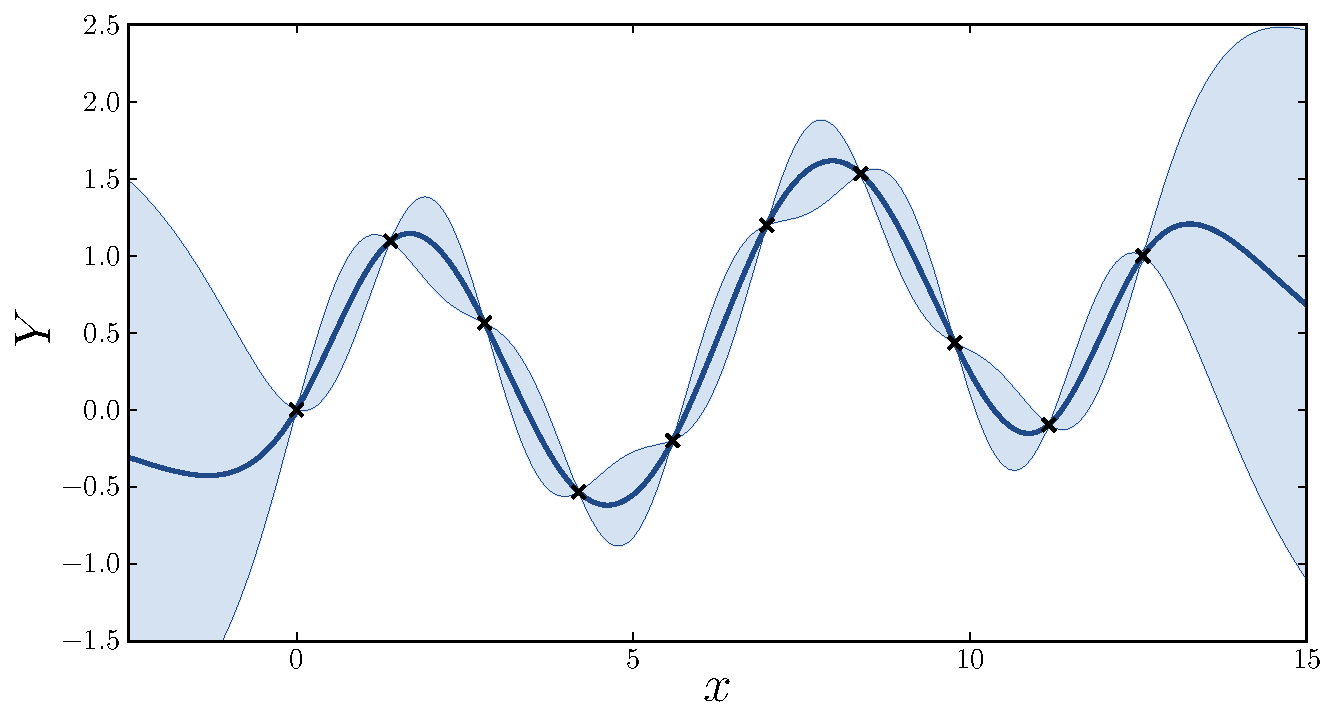
\includegraphics[height=6cm]{1_stat_models/figures/R/Fig1-GP}
\end{center}
\end{frame}

%%%%%%%%%%%%%%%%%%%%%%%%%%%%%%%%%%%%%%%%%%%%%%%%%%%%%%
\begin{frame}{}
A few remarkable properties of GPR models
\begin{itemize}
	\item They (can) interpolate the data-points
	\item The prediction variance does not depend on the observations
	\item The mean predictor does not depend on the variance
	\item They (usually) come back to zero when we are far away from the observations.
\end{itemize}
Can you prove them?
\end{frame}


%%%%%%%%%%%%%%%%%%%%%%%%%%%%%%%%%%%%%%%%%%%%%%%%%%%%%%
\begin{frame}{}
Changing the kernel \alert{has a huge impact on the model}:\\
\vspace{5mm}
\begin{center}
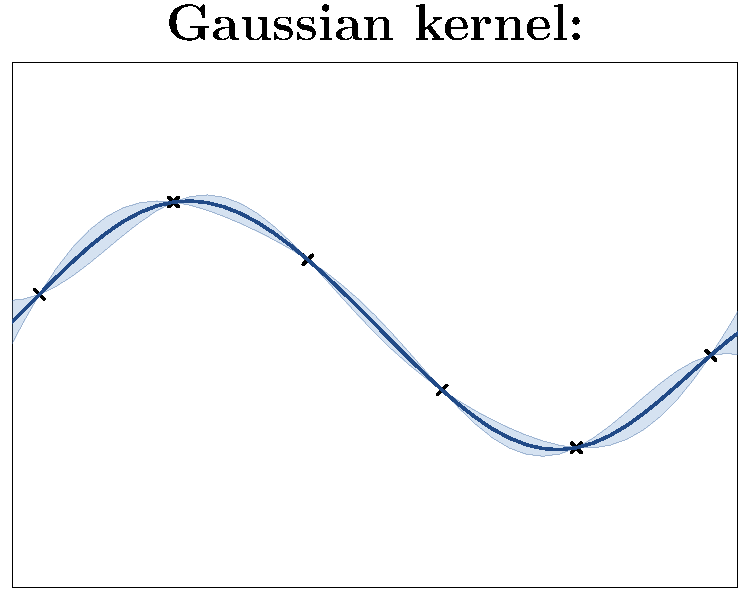
\includegraphics[height=3.9cm]{1_stat_models/figures/Fig2-GP-rbf} \qquad
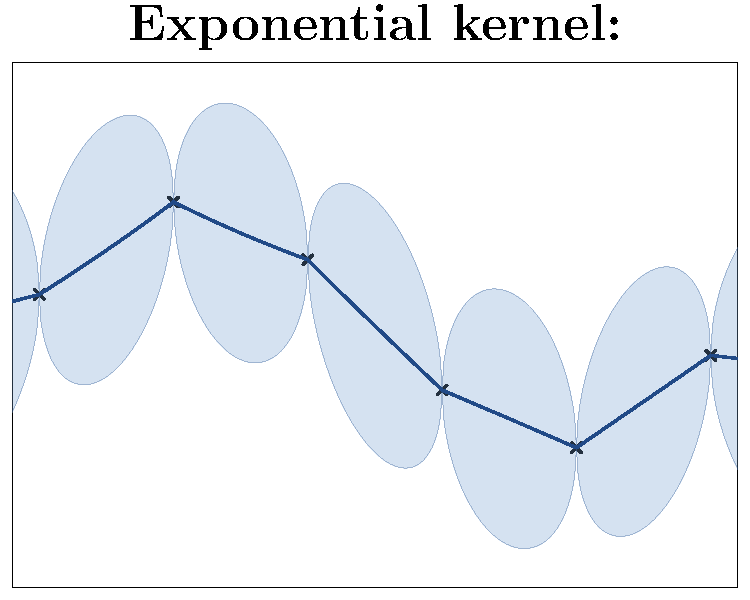
\includegraphics[height=3.9cm]{1_stat_models/figures/Fig2-GP-exp}
\end{center}
\end{frame}

%%%%%%%%%%%%%%%%%%%%%%%%%%%%%%%%%%%%%%%%%%%%%%%%%%%%%%
\begin{frame}{}
This is because changing the kernel means changing the prior on $f$\\
\vspace{5mm}
\begin{center}
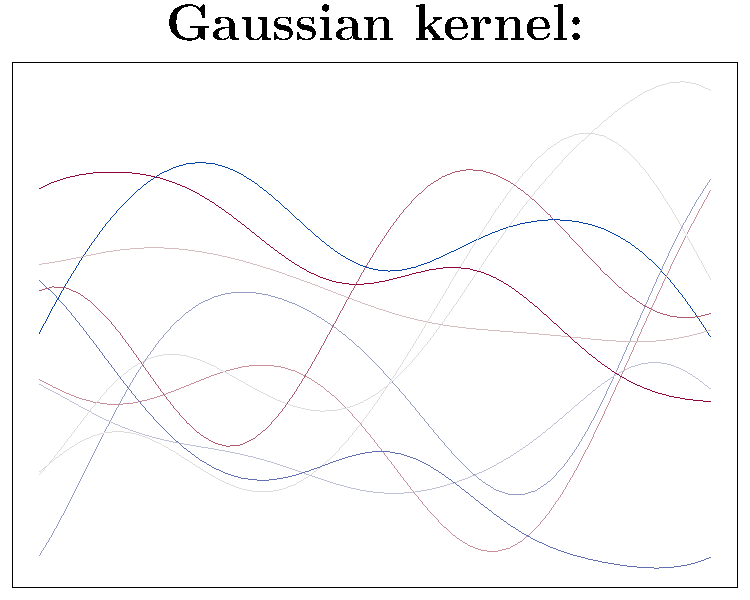
\includegraphics[height=3.8cm]{1_stat_models/figures/Fig2-sim-rbf} \qquad
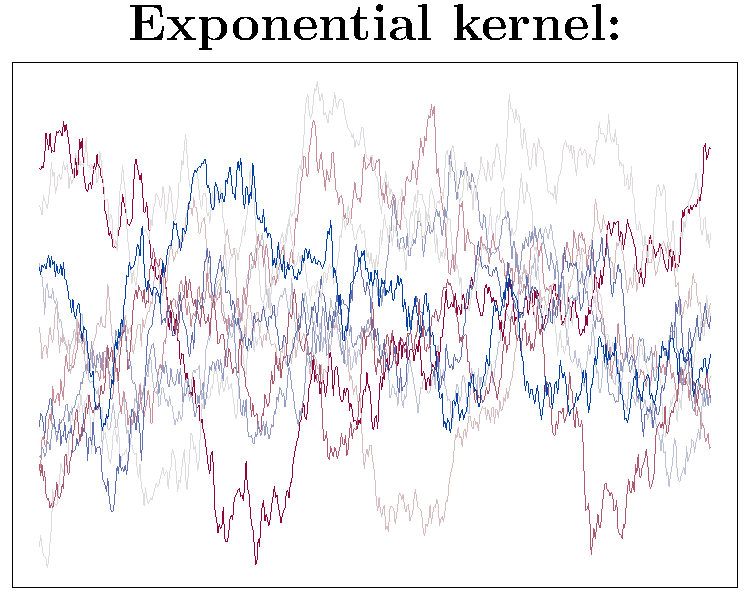
\includegraphics[height=3.8cm]{1_stat_models/figures/Fig2-sim-exp}
\end{center}
\end{frame}

%%%%%%%%%%%%%%%%%%%%%%%%%%%%%%%%%%%%%%%%%%%%%%%%%%%%%%
\begin{frame}{}
There is no model/kernel that is intrinsically better... it depends on the data!
\begin{center}
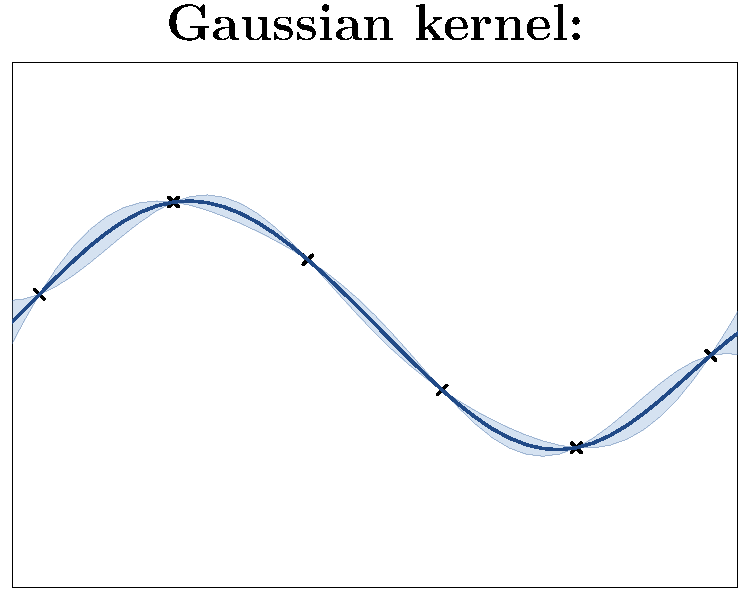
\includegraphics[height=3.5cm]{1_stat_models/figures/Fig2-GP-rbf} \hspace{1cm}
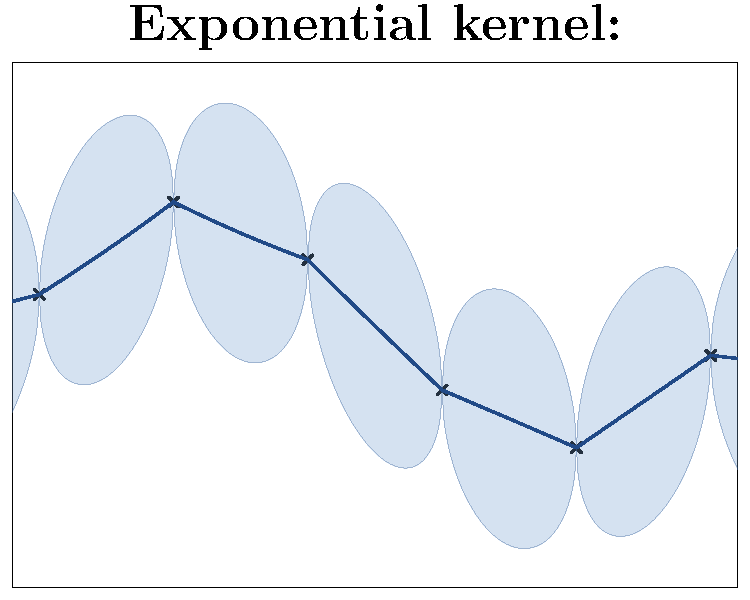
\includegraphics[height=3.5cm]{1_stat_models/figures/Fig2-GP-exp}
\end{center}
The kernel has to be chosen accordingly to our prior belief on the behaviour of the function to study:
\begin{itemize}
  \item is it continuous, differentiable, how many times?
  \item is it stationary ?
  \item ...
\end{itemize}
\end{frame}

%%%%%%%%%%%%%%%%%%%%%%%%%%%%%%%%%%%%%%%%%%%%%%%%%%%%%%
\begin{frame}{}
The best predictor can be seen either as a linear combination of
\begin{itemize}
	\item the observations: $m(x)=\alpha^t F$
	\item the kernel evaluated at $X$: $m(x)=k(x,X) \beta$
\end{itemize}
The later is interesting to understand the model shape and behaviour. \\
\vspace{5mm}
For example, we have for a squared exponential kernel
\begin{center}
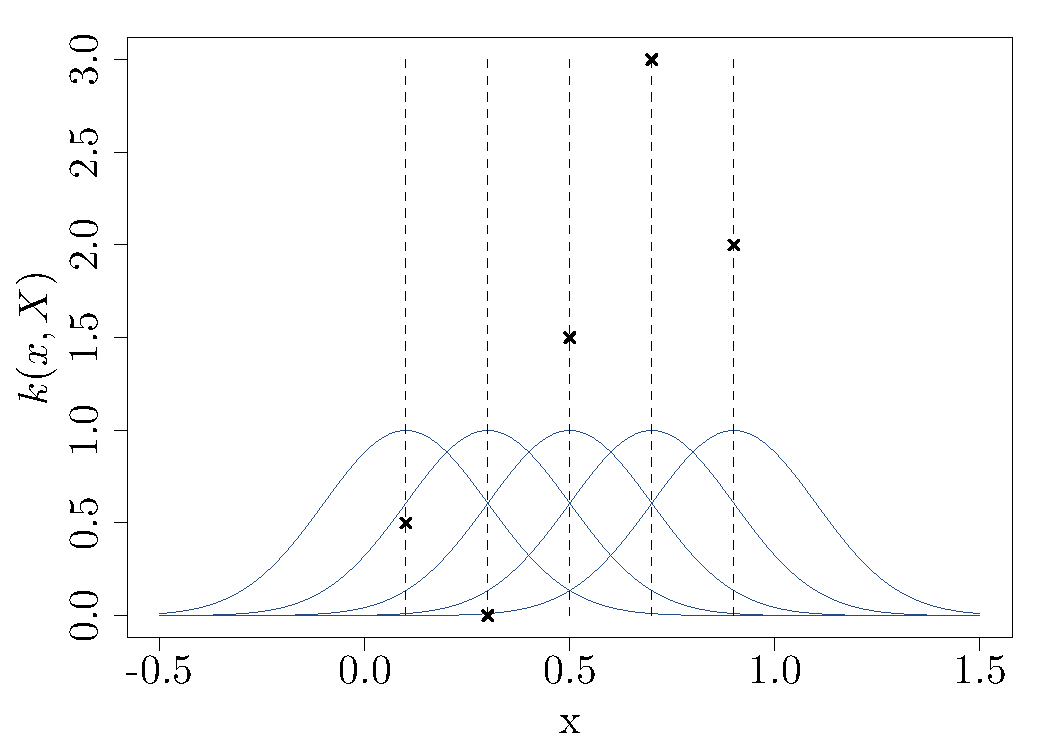
\includegraphics[height=4cm]{1_stat_models/figures/R/ch34_basisfuncGauss}
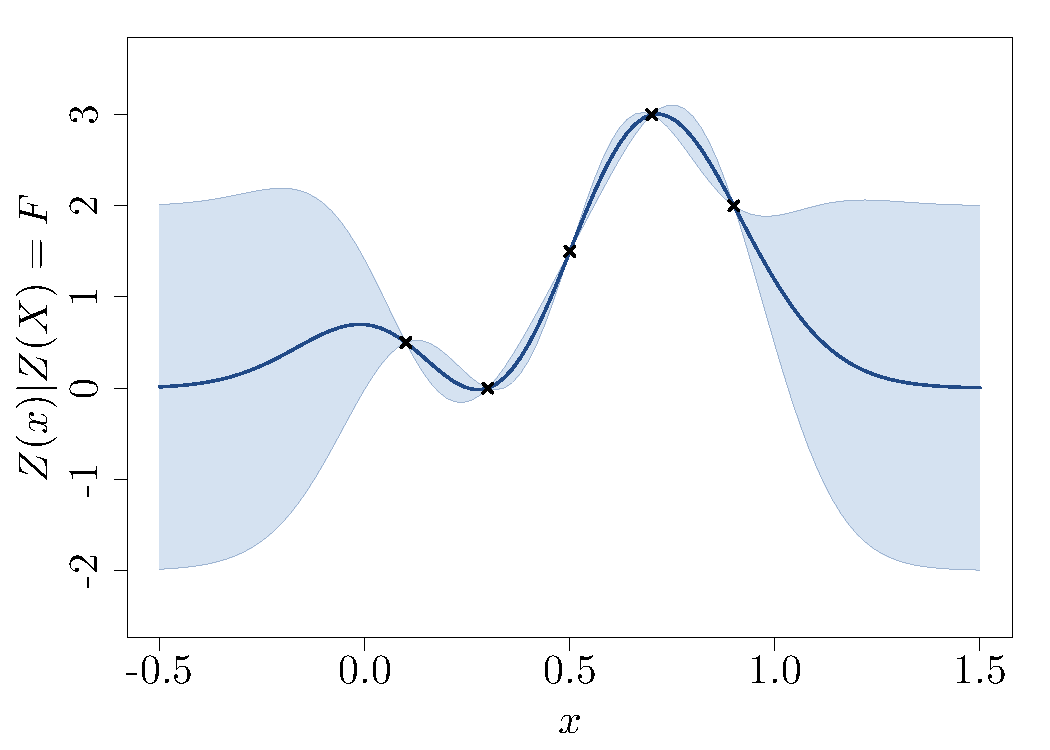
\includegraphics[height=4cm]{1_stat_models/figures/R/ch34_GPRbasisfuncGauss}
\end{center}
\end{frame}

%%%%%%%%%%%%%%%%%%%%%%%%%%%%%%%%%%%%%%%%%%%%%%%%%%%%%%
\begin{frame}{}
and for a Brownian kernel:
\begin{center}
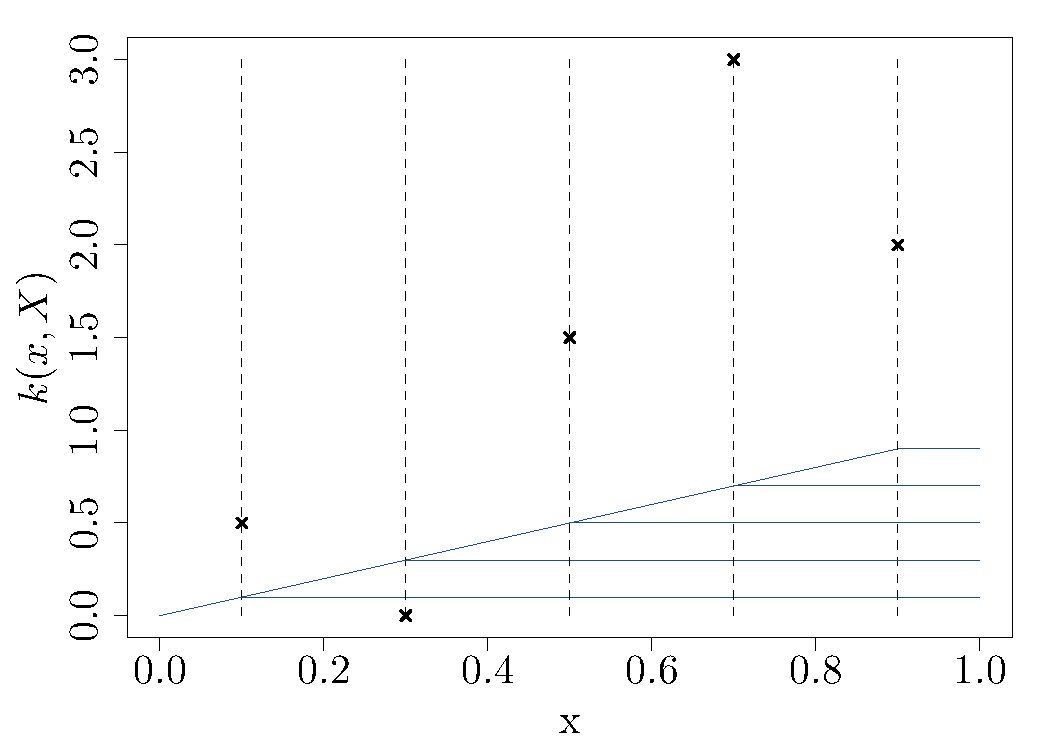
\includegraphics[height=4cm]{1_stat_models/figures/R/ch34_basisfuncBrown}
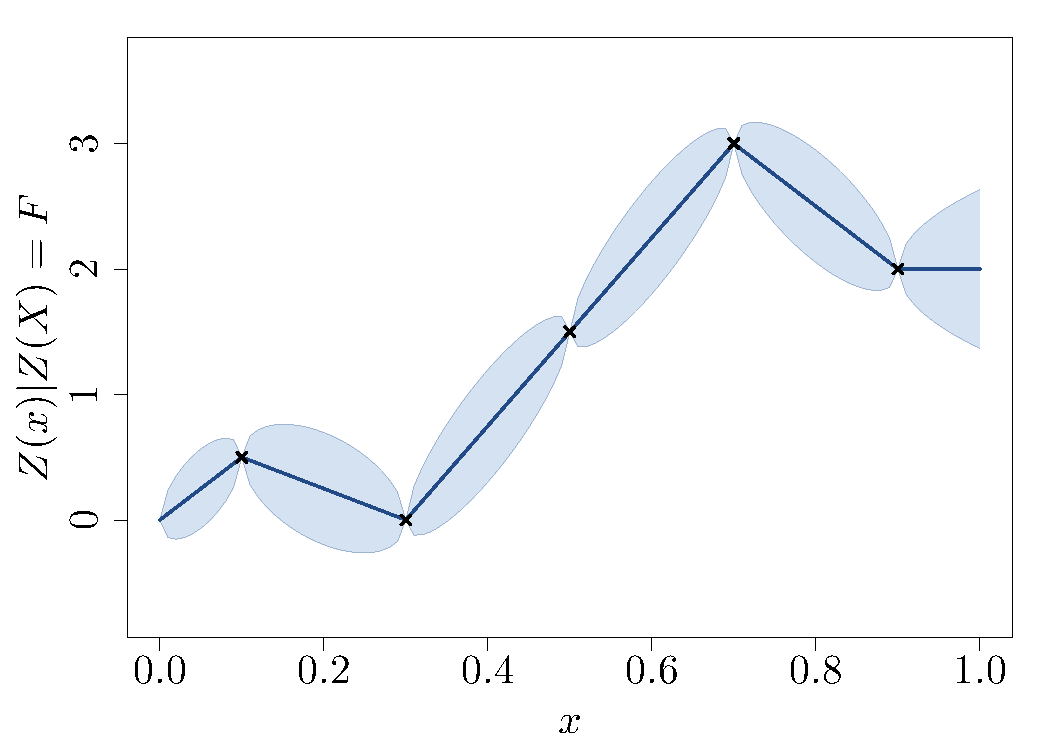
\includegraphics[height=4cm]{1_stat_models/figures/R/ch34_GPRbasisfuncBrown}
\end{center}
\end{frame}

%%%%%%%%%%%%%%%%%%%%%%%%%%%%%%%%%%%%%%%%%%%%%%%%%%%%%%
\begin{frame}{}
We are not always interested in models that interpolate the data. For example, if there is some observation noise: $F = f(X) + \varepsilon$.
% \begin{equation*}
% 	F = f(X) + \varepsilon
% \end{equation*}
% What would change in the model expression?
% \end{frame}

% %%%%%%%%%%%%%%%%%%%%%%%%%%%%%%%%%%%%%%%%%%%%%%%%%%%%%%
% \begin{frame}{}
\vspace{5mm}
Let $N$ be a process $\mathcal{N}(0,n)$ that represent the observation noise. The expressions of GPR with noise are
\begin{equation*}
	\begin{split}
	m(x) &= \E[Z(x)|Z(X) + N(X) \shorteq F] \\
	&= k(x,X) (k(X,X)+n(X,X))^{-1} F \\
	& \\
	c(x,y) &= \Cov[Z(x),Z(y)|Z(X)+ N(X) \shorteq F] \\
	&= k(x,y) - k(x,X) (k(X,X)+n(X,X))^{-1} k(X,y)
\end{split}
\end{equation*}
\end{frame}

%%%%%%%%%%%%%%%%%%%%%%%%%%%%%%%%%%%%%%%%%%%%%%%%%%%%%%
\begin{frame}{}
Examples of models with observation noise for $n(x,y)=\tau^2 \delta_{x,y}$:
\begin{center}
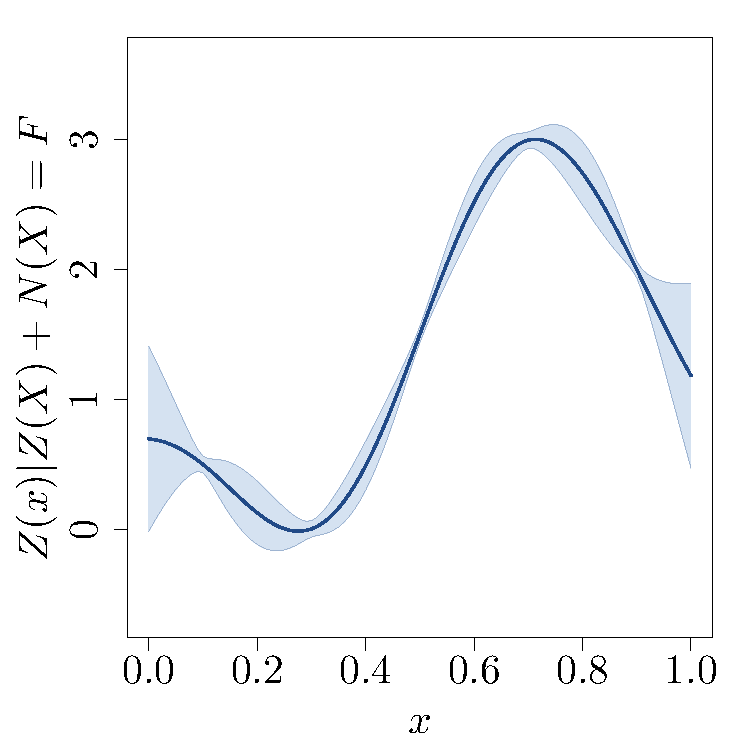
\includegraphics[height=3.5cm]{1_stat_models/figures/R/ch34_GPRnoise0001}
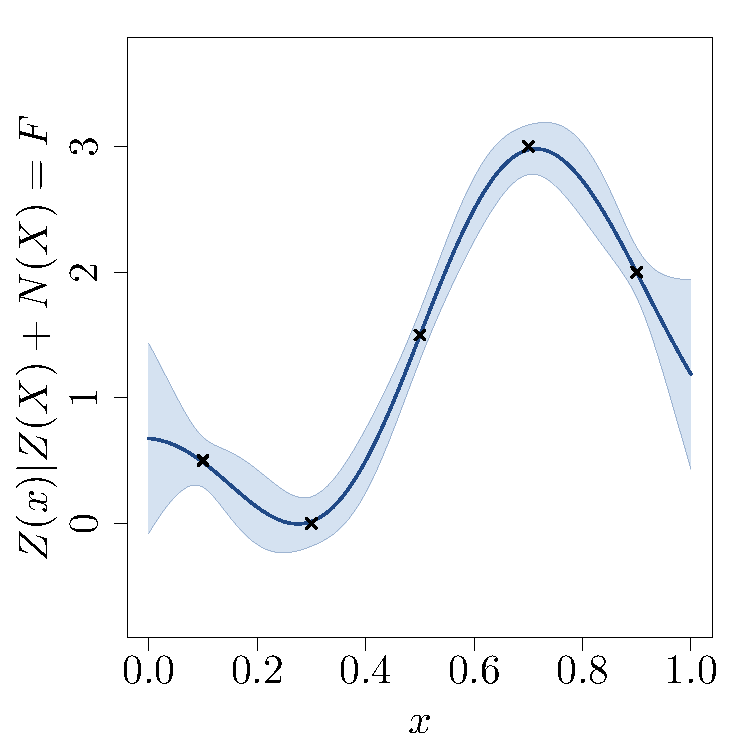
\includegraphics[height=3.5cm]{1_stat_models/figures/R/ch34_GPRnoise001}
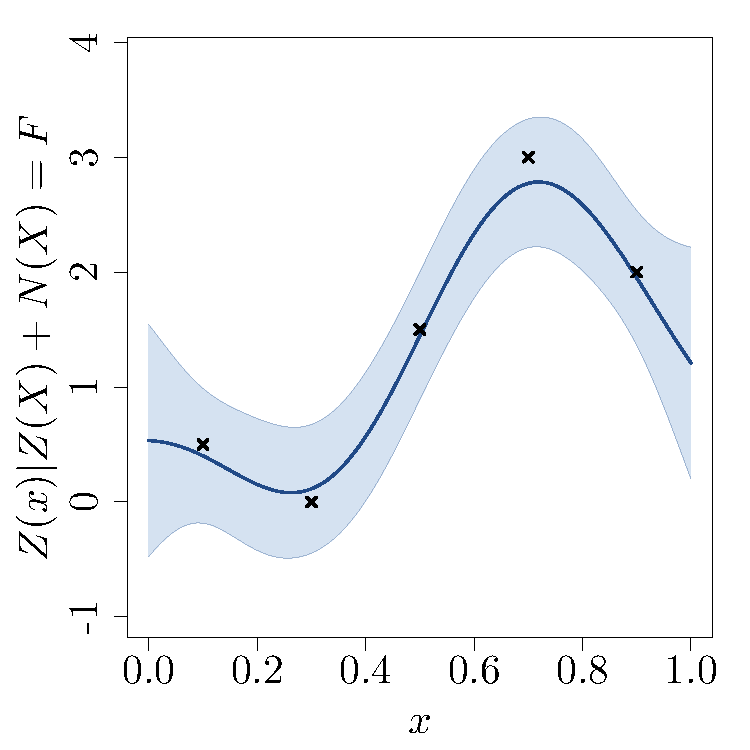
\includegraphics[height=3.5cm]{1_stat_models/figures/R/ch34_GPRnoise01}\\
The values of $\tau^2$ are respectively 0.001, 0.01 and 0.1.
\end{center}
\end{frame}

